% Chapter 12: Scoring models
% Statistics of Financial Markets -- Bachelor's programme, Bucharest University of Economic Studies
% GENERATED by latex/build_chapter12.py -- edit the generator, not this file.

\newcommand{\coursename}{Statistics of Financial Markets}
% Preambul comun SFM -- Statistica piețelor financiare / Statistics of Financial Markets (Beamer, 16:9)
% Același design ca MFM. Înainte de % Preambul comun SFM -- Statistica piețelor financiare / Statistics of Financial Markets (Beamer, 16:9)
% Același design ca MFM. Înainte de % Preambul comun SFM -- Statistica piețelor financiare / Statistics of Financial Markets (Beamer, 16:9)
% Același design ca MFM. Înainte de \input{../../latex/preamble} se definește
%   \newcommand{\coursename}{Statistics of Financial Markets}      (EN)
%   \newcommand{\coursename}{Statistica piețelor financiare}       (RO)  și  \def\sfmlang{ro}
% Fișierele .tex se află în EN/Courses, EN/Seminars, RO/Cursuri, RO/Seminarii (două niveluri sub rădăcină).
% Deck-urile sînt generate de latex/build_chapterN.py / build_seminarN.py (vezi latex/sfm_build.py).

\documentclass[9pt, aspectratio=169, t]{beamer}
\providecommand{\coursename}{Statistics of Financial Markets}

% Ensure content fits on slides
\setbeamersize{text margin left=8mm, text margin right=8mm}

%=============================================================================
% THEME AND STYLE CONFIGURATION
%=============================================================================
\usetheme{default}
% Using default theme for clean header/footer control

% Color Palette (matching Redispatch PDF)
\definecolor{MainBlue}{RGB}{26, 58, 110}
\definecolor{AccentBlue}{RGB}{26, 58, 110}
\definecolor{IDAred}{RGB}{205, 0, 0}
\definecolor{DarkGray}{RGB}{51, 51, 51}
\definecolor{MediumGray}{RGB}{128, 128, 128}
\definecolor{LightGray}{RGB}{248, 248, 248}
\definecolor{VeryLightGray}{RGB}{235, 235, 235}
\definecolor{KeynoteGray}{RGB}{218, 218, 218}
\definecolor{SectionGray}{RGB}{120, 120, 120}
\definecolor{FooterGray}{RGB}{100, 100, 100}
\definecolor{Crimson}{RGB}{220, 53, 69}
\definecolor{Forest}{RGB}{46, 125, 50}
\definecolor{Amber}{RGB}{181, 133, 63}
\definecolor{Orange}{RGB}{230, 126, 34}
\definecolor{Purple}{RGB}{142, 68, 173}

% Gradient background (exact Keynote 315° gradient: white to RGB 218,218,218)
\setbeamertemplate{background}{%
    \begin{tikzpicture}[remember picture, overlay]
        \shade[shading=axis, shading angle=315,
        top color=white, bottom color=KeynoteGray]
        (current page.south west) rectangle (current page.north east);
    \end{tikzpicture}%
}
% Fallback solid color for compatibility
\setbeamercolor{background canvas}{bg=}

\setbeamercolor{palette primary}{bg=MainBlue, fg=white}
\setbeamercolor{palette secondary}{bg=MainBlue!85, fg=white}
\setbeamercolor{palette tertiary}{bg=MainBlue!70, fg=white}
\setbeamercolor{structure}{fg=MainBlue}
\setbeamercolor{title}{fg=IDAred}
\setbeamercolor{frametitle}{fg=IDAred, bg=}
\setbeamercolor{block title}{bg=MainBlue, fg=white}
\setbeamercolor{block body}{bg=VeryLightGray, fg=DarkGray}
\setbeamercolor{block title alerted}{bg=Crimson, fg=white}
\setbeamercolor{block body alerted}{bg=Crimson!8, fg=DarkGray}
\setbeamercolor{block title example}{bg=Forest, fg=white}
\setbeamercolor{block body example}{bg=Forest!8, fg=DarkGray}
\setbeamercolor{item}{fg=MainBlue}

% Footer colors (override Madrid theme blue)
\setbeamercolor{author in head/foot}{fg=FooterGray, bg=}
\setbeamercolor{title in head/foot}{fg=FooterGray, bg=}
\setbeamercolor{date in head/foot}{fg=FooterGray, bg=}
\setbeamercolor{section in head/foot}{fg=FooterGray, bg=}
\setbeamercolor{subsection in head/foot}{fg=FooterGray, bg=}

% Bullet styles (apply everywhere including blocks)
\setbeamertemplate{itemize item}{\color{MainBlue}$\boxdot$}
\setbeamertemplate{itemize subitem}{\color{MainBlue}$\blacktriangleright$}
\setbeamertemplate{itemize subsubitem}{\color{MainBlue}\tiny$\bullet$}
\setbeamertemplate{itemize/enumerate body begin}{\normalsize}
\setbeamertemplate{itemize/enumerate subbody begin}{\normalsize}

% Item spacing - compact style
\setlength{\leftmargini}{10pt}       % Level 1: minimal indent
\setlength{\leftmarginii}{10pt}      % Level 2: minimal additional indent
% Compact list spacing (zero extra space before/after lists in blocks)
\makeatletter
\def\@listi{\leftmargin\leftmargini \topsep 0pt \parsep 0pt \itemsep 0pt}
\def\@listii{\leftmargin\leftmarginii \topsep 0pt \parsep 0pt \itemsep 0pt}
\makeatother

\setbeamertemplate{navigation symbols}{}

%=============================================================================
% CUSTOM HEADLINE
%=============================================================================
\setbeamertemplate{headline}{%
    \vskip10pt%
    \hbox to \paperwidth{%
        \hskip0.5cm%
        {\small\color{FooterGray}\renewcommand{\hyperlink}[2]{##2}\insertsectionhead}%
        \hfill%
        \textcolor{FooterGray}{\small\insertframenumber}%
        \hskip0.5cm%
    }%
    \vskip4pt%
    {\color{FooterGray}\hrule height 0.4pt}%
}

%=============================================================================
% CUSTOM FOOTER
%=============================================================================
\usepackage{fontawesome5}

\setbeamertemplate{footline}{%
    {\color{FooterGray}\hrule height 0.4pt}%
    \vskip4pt%
    \hbox to \paperwidth{%
        \hskip0.5cm%
        \textcolor{FooterGray}{\small\coursename}%
        \hfill%
        \raisebox{-0.1em}{%
            \begin{tikzpicture}[x=0.08em, y=0.08em, line width=0.4pt]
                \draw[FooterGray] (0,3) -- (1,4) -- (2,3.5) -- (3,5) -- (4,4) -- (5,6) -- (6,5.5) -- (7,4) -- (8,5) -- (9,7) -- (10,6) -- (11,5) -- (12,6.5) -- (13,8) -- (14,7) -- (15,6) -- (16,7.5) -- (17,9) -- (18,8) -- (19,7) -- (20,8.5) -- (21,10) -- (22,9) -- (23,8) -- (24,9.5);
            \end{tikzpicture}%
        }%
        \hskip0.5cm%
    }%
    \vskip6pt%
}

%=============================================================================
% PACKAGES
%=============================================================================
\usepackage[utf8]{inputenc}
\DeclareUnicodeCharacter{03B1}{\ensuremath{\alpha}}
\usepackage[T1]{fontenc}
\usepackage{amsmath, amssymb, amsthm}
\usepackage{mathtools}
\usepackage{bm}
\usepackage{tikz}
\usetikzlibrary{arrows.meta, positioning, shapes, calc, decorations.pathreplacing, shadings}
\usepackage{booktabs}
\usepackage{multirow}
\usepackage{array}
\usepackage{graphicx}
\usepackage{hyperref}
\usepackage{colortbl}
\usepackage{listings}
\lstset{language=Python, basicstyle=\ttfamily\scriptsize, keywordstyle=\color{MainBlue}\bfseries,
  commentstyle=\color{Forest}, stringstyle=\color{Crimson}, breaklines=true,
  frame=none, backgroundcolor=\color{VeryLightGray}, xleftmargin=2mm}
\hypersetup{colorlinks=true, linkcolor=MainBlue, urlcolor=MainBlue}
\graphicspath{{../../logos/}{../../charts/}{../../photos/}}
\usepackage{xcolor}
\hfuzz=2pt  % Suppress tiny overfull warnings (<2pt)
\vfuzz=2pt  % Suppress tiny vertical overfull warnings (<2pt)

%=============================================================================
% QUANTLET COMMANDS
%   \quantlet{<displayed name>}{<url>}       (generic, compatible with the older SFM decks)
%   \sfmquantlet{Ch_05}{SFM_ch5_garch}       -> https://github.com/danpele/SFM/tree/main/Quantlets/Ch_05/SFM_ch5_garch
%   \qlurl{<folder>} is defined per chapter by the generator (Quantlets/Ch_NN/<folder>)
%=============================================================================
\newcommand{\sfmrepo}{https://github.com/danpele/SFM}
\newcommand{\sfmqlbase}{https://github.com/danpele/SFM/tree/main/Quantlets}
\newcommand{\quantlet}[2]{%
    \hfill\href{#2}{%
        \raisebox{-0.15em}{
\includegraphics[height=0.7em]{ql_logo.png}}%
        \textcolor{MainBlue}{\tiny\ #1}%
    }%
}
\newcommand{\sfmquantlet}[2]{\quantlet{\detokenize{#2}}{\sfmqlbase/#1/#2}}

%=============================================================================
% NOTEBOOKS (Google Colab)
%   \colaburl{notebooks/EN/chapter5_seminar_notebook.ipynb} -> the Colab link of a file in the SFM repo
%   \nb: the chapter notebook (each seminar deck redefines it with \renewcommand)
%=============================================================================
\newcommand{\colaburl}[1]{https://colab.research.google.com/github/danpele/SFM/blob/main/#1}
\newcommand{\nb}{https://colab.research.google.com/github/danpele/SFM/tree/main/notebooks/EN}
\newcommand{\nbname}{notebooks/EN}

%=============================================================================
% SLIDE HELPERS (used by the generators; the same as in MFM)
%=============================================================================
% local font size for list bodies (the preamble forces \normalsize)
\newcommand{\itemsize}[1]{\setbeamertemplate{itemize/enumerate body begin}{#1}\setbeamertemplate{itemize/enumerate subbody begin}{#1}}
\newcommand{\intitle}[1]{{\hypersetup{urlcolor=white}#1}}   % white links inside coloured title bars
\newcommand{\imgcap}[1]{{\scriptsize #1}\\[0.5mm]}          % caption under a photo
\newcommand{\imgcredit}[2]{{\tiny\color{FooterGray}\href{#1}{#2}}}   % image credit: source URL, author/licence
\newcommand{\aiprompt}[1]{{\ttfamily\color{MainBlue}#1}}     % a prompt to an AI assistant

%=============================================================================
% SEMINARS: student version by default; the instructor wrapper *_solutions.tex sets \solutionstrue
%=============================================================================
\makeatletter\@ifundefined{ifsolutions}{\expandafter\newif\csname ifsolutions\endcsname}{}\makeatother
\newcommand{\solonly}[1]{\ifsolutions #1\fi}
\newcommand{\propsub}{\ifsolutions\else\framesubtitle{\ifdefined\sfmlang Rezolvarea se discută la seminar\else Solution discussed in class\fi}\fi}

%=============================================================================
% APPENDIX AND CHAPTER LINKS (latex/appendix_links.py writes the calls; it also re-declares these
% macros before \begin{document}, so the decks compile with or without this preamble block)
%=============================================================================
\providecommand{\sfmapplink}[3]{\hypertarget{#2}{}\hyperlink{#1}{\beamergotobutton{#3}}}
\providecommand{\sfmappback}[2]{\begin{tikzpicture}[remember picture,overlay]\node[anchor=south east] at ([xshift=-3mm,yshift=7mm]current page.south east){\hyperlink{#1}{\beamerreturnbutton{#2}}};\end{tikzpicture}}
\providecommand{\sfmchlink}[2]{\href{#1}{#2}}
\providecommand{\sfmchlinkt}[2]{\href{#1}{\usebeamercolor[fg]{frametitle}#2}}

%=============================================================================
% QUANTINAR COMMAND: link către un curs Quantinar (subiecte avansate)
%=============================================================================
\newcommand{\quantinar}[2]{%
    \href{#2}{%
        \raisebox{-0.15em}{
\includegraphics[height=0.8em]{qr_logo.png}}%
        \textcolor{MainBlue}{\scriptsize\ #1}%
    }%
}

%=============================================================================
% CUSTOM TITLE PAGE
%=============================================================================
\defbeamertemplate*{title page}{hybrid}[1][]
{
    \vspace{0.2cm}
    % Logos row - top header (with clickable links)
    \begin{center}
        \href{https://www.ase.ro}{
\includegraphics[height=1.0cm]{ase_logo.png}}\hspace{0.3cm}%
        \href{https://theida.net}{
\includegraphics[height=1.0cm]{ida_logo.png}}\hspace{0.3cm}%
        \href{https://blockchain-research-center.com}{
\includegraphics[height=1.0cm]{brc_logo.png}}\hspace{0.3cm}%
        \href{https://www.ai4efin.ase.ro}{
\includegraphics[height=1.0cm]{ai4efin_logo.png}}\hspace{0.3cm}%
        \href{https://ipe.ro/new}{
\includegraphics[height=1.0cm]{acad_logo.png}}\hspace{0.3cm}%
        \href{https://www.digital-finance-msca.com}{
\includegraphics[height=1.0cm]{msca_logo.png}}%
    \end{center}

    \vspace{0.6cm}

    % Main title with Q logos on sides (with clickable links)
    \begin{center}
        \begin{minipage}{0.1\textwidth}
            \centering
            \href{https://quantlet.com}{
\includegraphics[height=1.1cm]{ql_logo.png}}
        \end{minipage}%
        \begin{minipage}{0.78\textwidth}
            \centering
            {\LARGE\bfseries\usebeamercolor[fg]{title}\inserttitle}

            \vspace{0.3cm}

            {\usebeamerfont{subtitle}\usebeamercolor[fg]{title}\insertsubtitle}
        \end{minipage}%
        \begin{minipage}{0.1\textwidth}
            \centering
            \href{https://quantinar.com}{
\includegraphics[height=1.1cm]{qr_logo.png}}
        \end{minipage}
    \end{center}

    \vspace{0.6cm}

    % Authors (left aligned)
    \hspace{0.5cm}{\usebeamerfont{author}\insertauthor}

    \vspace{0.3cm}

    % Institute/Affiliations (left aligned)
    \hspace{0.5cm}\begin{minipage}[t]{0.9\textwidth}
        \raggedright\small\insertinstitute
    \end{minipage}
}

%=============================================================================
% THEOREM ENVIRONMENTS
%=============================================================================
\theoremstyle{definition}
\setbeamertemplate{theorems}[numbered]
\ifdefined\sfmlang
\newtheorem{defn}{Definiție}
\newtheorem{thm}{Teoremă}
\newtheorem{prop}{Propoziție}
\newtheorem{rmk}{Observație}
\else
\newtheorem{defn}{Definition}
\newtheorem{thm}{Theorem}
\newtheorem{prop}{Proposition}
\newtheorem{rmk}{Remark}
\fi

%=============================================================================
% CENTRED MINIPAGE (no extra vertical space)
%=============================================================================
\newenvironment{cminipage}[1]{%
    \par\noindent\hfill\begin{minipage}{#1}\ignorespaces
}{%
    \end{minipage}\hfill\null\par
}

%=============================================================================
% CUSTOM COMMANDS
%=============================================================================
\newcommand{\E}{\mathbb{E}}
\newcommand{\Var}{\text{Var}}
\newcommand{\Cov}{\text{Cov}}
\newcommand{\Corr}{\text{Corr}}
\newcommand{\R}{\mathbb{R}}
\newcommand{\N}{\mathbb{N}}
\newcommand{\Z}{\mathbb{Z}}
\newcommand{\B}{\mathbf{B}}
\newcommand{\imark}{\textcolor{MainBlue}{\textbullet}}
\newcommand{\RMSE}{\text{RMSE}}
\newcommand{\MAE}{\text{MAE}}
\newcommand{\MAPE}{\text{MAPE}}

 se definește
%   \newcommand{\coursename}{Statistics of Financial Markets}      (EN)
%   \newcommand{\coursename}{Statistica piețelor financiare}       (RO)  și  \def\sfmlang{ro}
% Fișierele .tex se află în EN/Courses, EN/Seminars, RO/Cursuri, RO/Seminarii (două niveluri sub rădăcină).
% Deck-urile sînt generate de latex/build_chapterN.py / build_seminarN.py (vezi latex/sfm_build.py).

\documentclass[9pt, aspectratio=169, t]{beamer}
\providecommand{\coursename}{Statistics of Financial Markets}

% Ensure content fits on slides
\setbeamersize{text margin left=8mm, text margin right=8mm}

%=============================================================================
% THEME AND STYLE CONFIGURATION
%=============================================================================
\usetheme{default}
% Using default theme for clean header/footer control

% Color Palette (matching Redispatch PDF)
\definecolor{MainBlue}{RGB}{26, 58, 110}
\definecolor{AccentBlue}{RGB}{26, 58, 110}
\definecolor{IDAred}{RGB}{205, 0, 0}
\definecolor{DarkGray}{RGB}{51, 51, 51}
\definecolor{MediumGray}{RGB}{128, 128, 128}
\definecolor{LightGray}{RGB}{248, 248, 248}
\definecolor{VeryLightGray}{RGB}{235, 235, 235}
\definecolor{KeynoteGray}{RGB}{218, 218, 218}
\definecolor{SectionGray}{RGB}{120, 120, 120}
\definecolor{FooterGray}{RGB}{100, 100, 100}
\definecolor{Crimson}{RGB}{220, 53, 69}
\definecolor{Forest}{RGB}{46, 125, 50}
\definecolor{Amber}{RGB}{181, 133, 63}
\definecolor{Orange}{RGB}{230, 126, 34}
\definecolor{Purple}{RGB}{142, 68, 173}

% Gradient background (exact Keynote 315° gradient: white to RGB 218,218,218)
\setbeamertemplate{background}{%
    \begin{tikzpicture}[remember picture, overlay]
        \shade[shading=axis, shading angle=315,
        top color=white, bottom color=KeynoteGray]
        (current page.south west) rectangle (current page.north east);
    \end{tikzpicture}%
}
% Fallback solid color for compatibility
\setbeamercolor{background canvas}{bg=}

\setbeamercolor{palette primary}{bg=MainBlue, fg=white}
\setbeamercolor{palette secondary}{bg=MainBlue!85, fg=white}
\setbeamercolor{palette tertiary}{bg=MainBlue!70, fg=white}
\setbeamercolor{structure}{fg=MainBlue}
\setbeamercolor{title}{fg=IDAred}
\setbeamercolor{frametitle}{fg=IDAred, bg=}
\setbeamercolor{block title}{bg=MainBlue, fg=white}
\setbeamercolor{block body}{bg=VeryLightGray, fg=DarkGray}
\setbeamercolor{block title alerted}{bg=Crimson, fg=white}
\setbeamercolor{block body alerted}{bg=Crimson!8, fg=DarkGray}
\setbeamercolor{block title example}{bg=Forest, fg=white}
\setbeamercolor{block body example}{bg=Forest!8, fg=DarkGray}
\setbeamercolor{item}{fg=MainBlue}

% Footer colors (override Madrid theme blue)
\setbeamercolor{author in head/foot}{fg=FooterGray, bg=}
\setbeamercolor{title in head/foot}{fg=FooterGray, bg=}
\setbeamercolor{date in head/foot}{fg=FooterGray, bg=}
\setbeamercolor{section in head/foot}{fg=FooterGray, bg=}
\setbeamercolor{subsection in head/foot}{fg=FooterGray, bg=}

% Bullet styles (apply everywhere including blocks)
\setbeamertemplate{itemize item}{\color{MainBlue}$\boxdot$}
\setbeamertemplate{itemize subitem}{\color{MainBlue}$\blacktriangleright$}
\setbeamertemplate{itemize subsubitem}{\color{MainBlue}\tiny$\bullet$}
\setbeamertemplate{itemize/enumerate body begin}{\normalsize}
\setbeamertemplate{itemize/enumerate subbody begin}{\normalsize}

% Item spacing - compact style
\setlength{\leftmargini}{10pt}       % Level 1: minimal indent
\setlength{\leftmarginii}{10pt}      % Level 2: minimal additional indent
% Compact list spacing (zero extra space before/after lists in blocks)
\makeatletter
\def\@listi{\leftmargin\leftmargini \topsep 0pt \parsep 0pt \itemsep 0pt}
\def\@listii{\leftmargin\leftmarginii \topsep 0pt \parsep 0pt \itemsep 0pt}
\makeatother

\setbeamertemplate{navigation symbols}{}

%=============================================================================
% CUSTOM HEADLINE
%=============================================================================
\setbeamertemplate{headline}{%
    \vskip10pt%
    \hbox to \paperwidth{%
        \hskip0.5cm%
        {\small\color{FooterGray}\renewcommand{\hyperlink}[2]{##2}\insertsectionhead}%
        \hfill%
        \textcolor{FooterGray}{\small\insertframenumber}%
        \hskip0.5cm%
    }%
    \vskip4pt%
    {\color{FooterGray}\hrule height 0.4pt}%
}

%=============================================================================
% CUSTOM FOOTER
%=============================================================================
\usepackage{fontawesome5}

\setbeamertemplate{footline}{%
    {\color{FooterGray}\hrule height 0.4pt}%
    \vskip4pt%
    \hbox to \paperwidth{%
        \hskip0.5cm%
        \textcolor{FooterGray}{\small\coursename}%
        \hfill%
        \raisebox{-0.1em}{%
            \begin{tikzpicture}[x=0.08em, y=0.08em, line width=0.4pt]
                \draw[FooterGray] (0,3) -- (1,4) -- (2,3.5) -- (3,5) -- (4,4) -- (5,6) -- (6,5.5) -- (7,4) -- (8,5) -- (9,7) -- (10,6) -- (11,5) -- (12,6.5) -- (13,8) -- (14,7) -- (15,6) -- (16,7.5) -- (17,9) -- (18,8) -- (19,7) -- (20,8.5) -- (21,10) -- (22,9) -- (23,8) -- (24,9.5);
            \end{tikzpicture}%
        }%
        \hskip0.5cm%
    }%
    \vskip6pt%
}

%=============================================================================
% PACKAGES
%=============================================================================
\usepackage[utf8]{inputenc}
\DeclareUnicodeCharacter{03B1}{\ensuremath{\alpha}}
\usepackage[T1]{fontenc}
\usepackage{amsmath, amssymb, amsthm}
\usepackage{mathtools}
\usepackage{bm}
\usepackage{tikz}
\usetikzlibrary{arrows.meta, positioning, shapes, calc, decorations.pathreplacing, shadings}
\usepackage{booktabs}
\usepackage{multirow}
\usepackage{array}
\usepackage{graphicx}
\usepackage{hyperref}
\usepackage{colortbl}
\usepackage{listings}
\lstset{language=Python, basicstyle=\ttfamily\scriptsize, keywordstyle=\color{MainBlue}\bfseries,
  commentstyle=\color{Forest}, stringstyle=\color{Crimson}, breaklines=true,
  frame=none, backgroundcolor=\color{VeryLightGray}, xleftmargin=2mm}
\hypersetup{colorlinks=true, linkcolor=MainBlue, urlcolor=MainBlue}
\graphicspath{{../../logos/}{../../charts/}{../../photos/}}
\usepackage{xcolor}
\hfuzz=2pt  % Suppress tiny overfull warnings (<2pt)
\vfuzz=2pt  % Suppress tiny vertical overfull warnings (<2pt)

%=============================================================================
% QUANTLET COMMANDS
%   \quantlet{<displayed name>}{<url>}       (generic, compatible with the older SFM decks)
%   \sfmquantlet{Ch_05}{SFM_ch5_garch}       -> https://github.com/danpele/SFM/tree/main/Quantlets/Ch_05/SFM_ch5_garch
%   \qlurl{<folder>} is defined per chapter by the generator (Quantlets/Ch_NN/<folder>)
%=============================================================================
\newcommand{\sfmrepo}{https://github.com/danpele/SFM}
\newcommand{\sfmqlbase}{https://github.com/danpele/SFM/tree/main/Quantlets}
\newcommand{\quantlet}[2]{%
    \hfill\href{#2}{%
        \raisebox{-0.15em}{
\includegraphics[height=0.7em]{ql_logo.png}}%
        \textcolor{MainBlue}{\tiny\ #1}%
    }%
}
\newcommand{\sfmquantlet}[2]{\quantlet{\detokenize{#2}}{\sfmqlbase/#1/#2}}

%=============================================================================
% NOTEBOOKS (Google Colab)
%   \colaburl{notebooks/EN/chapter5_seminar_notebook.ipynb} -> the Colab link of a file in the SFM repo
%   \nb: the chapter notebook (each seminar deck redefines it with \renewcommand)
%=============================================================================
\newcommand{\colaburl}[1]{https://colab.research.google.com/github/danpele/SFM/blob/main/#1}
\newcommand{\nb}{https://colab.research.google.com/github/danpele/SFM/tree/main/notebooks/EN}
\newcommand{\nbname}{notebooks/EN}

%=============================================================================
% SLIDE HELPERS (used by the generators; the same as in MFM)
%=============================================================================
% local font size for list bodies (the preamble forces \normalsize)
\newcommand{\itemsize}[1]{\setbeamertemplate{itemize/enumerate body begin}{#1}\setbeamertemplate{itemize/enumerate subbody begin}{#1}}
\newcommand{\intitle}[1]{{\hypersetup{urlcolor=white}#1}}   % white links inside coloured title bars
\newcommand{\imgcap}[1]{{\scriptsize #1}\\[0.5mm]}          % caption under a photo
\newcommand{\imgcredit}[2]{{\tiny\color{FooterGray}\href{#1}{#2}}}   % image credit: source URL, author/licence
\newcommand{\aiprompt}[1]{{\ttfamily\color{MainBlue}#1}}     % a prompt to an AI assistant

%=============================================================================
% SEMINARS: student version by default; the instructor wrapper *_solutions.tex sets \solutionstrue
%=============================================================================
\makeatletter\@ifundefined{ifsolutions}{\expandafter\newif\csname ifsolutions\endcsname}{}\makeatother
\newcommand{\solonly}[1]{\ifsolutions #1\fi}
\newcommand{\propsub}{\ifsolutions\else\framesubtitle{\ifdefined\sfmlang Rezolvarea se discută la seminar\else Solution discussed in class\fi}\fi}

%=============================================================================
% APPENDIX AND CHAPTER LINKS (latex/appendix_links.py writes the calls; it also re-declares these
% macros before \begin{document}, so the decks compile with or without this preamble block)
%=============================================================================
\providecommand{\sfmapplink}[3]{\hypertarget{#2}{}\hyperlink{#1}{\beamergotobutton{#3}}}
\providecommand{\sfmappback}[2]{\begin{tikzpicture}[remember picture,overlay]\node[anchor=south east] at ([xshift=-3mm,yshift=7mm]current page.south east){\hyperlink{#1}{\beamerreturnbutton{#2}}};\end{tikzpicture}}
\providecommand{\sfmchlink}[2]{\href{#1}{#2}}
\providecommand{\sfmchlinkt}[2]{\href{#1}{\usebeamercolor[fg]{frametitle}#2}}

%=============================================================================
% QUANTINAR COMMAND: link către un curs Quantinar (subiecte avansate)
%=============================================================================
\newcommand{\quantinar}[2]{%
    \href{#2}{%
        \raisebox{-0.15em}{
\includegraphics[height=0.8em]{qr_logo.png}}%
        \textcolor{MainBlue}{\scriptsize\ #1}%
    }%
}

%=============================================================================
% CUSTOM TITLE PAGE
%=============================================================================
\defbeamertemplate*{title page}{hybrid}[1][]
{
    \vspace{0.2cm}
    % Logos row - top header (with clickable links)
    \begin{center}
        \href{https://www.ase.ro}{
\includegraphics[height=1.0cm]{ase_logo.png}}\hspace{0.3cm}%
        \href{https://theida.net}{
\includegraphics[height=1.0cm]{ida_logo.png}}\hspace{0.3cm}%
        \href{https://blockchain-research-center.com}{
\includegraphics[height=1.0cm]{brc_logo.png}}\hspace{0.3cm}%
        \href{https://www.ai4efin.ase.ro}{
\includegraphics[height=1.0cm]{ai4efin_logo.png}}\hspace{0.3cm}%
        \href{https://ipe.ro/new}{
\includegraphics[height=1.0cm]{acad_logo.png}}\hspace{0.3cm}%
        \href{https://www.digital-finance-msca.com}{
\includegraphics[height=1.0cm]{msca_logo.png}}%
    \end{center}

    \vspace{0.6cm}

    % Main title with Q logos on sides (with clickable links)
    \begin{center}
        \begin{minipage}{0.1\textwidth}
            \centering
            \href{https://quantlet.com}{
\includegraphics[height=1.1cm]{ql_logo.png}}
        \end{minipage}%
        \begin{minipage}{0.78\textwidth}
            \centering
            {\LARGE\bfseries\usebeamercolor[fg]{title}\inserttitle}

            \vspace{0.3cm}

            {\usebeamerfont{subtitle}\usebeamercolor[fg]{title}\insertsubtitle}
        \end{minipage}%
        \begin{minipage}{0.1\textwidth}
            \centering
            \href{https://quantinar.com}{
\includegraphics[height=1.1cm]{qr_logo.png}}
        \end{minipage}
    \end{center}

    \vspace{0.6cm}

    % Authors (left aligned)
    \hspace{0.5cm}{\usebeamerfont{author}\insertauthor}

    \vspace{0.3cm}

    % Institute/Affiliations (left aligned)
    \hspace{0.5cm}\begin{minipage}[t]{0.9\textwidth}
        \raggedright\small\insertinstitute
    \end{minipage}
}

%=============================================================================
% THEOREM ENVIRONMENTS
%=============================================================================
\theoremstyle{definition}
\setbeamertemplate{theorems}[numbered]
\ifdefined\sfmlang
\newtheorem{defn}{Definiție}
\newtheorem{thm}{Teoremă}
\newtheorem{prop}{Propoziție}
\newtheorem{rmk}{Observație}
\else
\newtheorem{defn}{Definition}
\newtheorem{thm}{Theorem}
\newtheorem{prop}{Proposition}
\newtheorem{rmk}{Remark}
\fi

%=============================================================================
% CENTRED MINIPAGE (no extra vertical space)
%=============================================================================
\newenvironment{cminipage}[1]{%
    \par\noindent\hfill\begin{minipage}{#1}\ignorespaces
}{%
    \end{minipage}\hfill\null\par
}

%=============================================================================
% CUSTOM COMMANDS
%=============================================================================
\newcommand{\E}{\mathbb{E}}
\newcommand{\Var}{\text{Var}}
\newcommand{\Cov}{\text{Cov}}
\newcommand{\Corr}{\text{Corr}}
\newcommand{\R}{\mathbb{R}}
\newcommand{\N}{\mathbb{N}}
\newcommand{\Z}{\mathbb{Z}}
\newcommand{\B}{\mathbf{B}}
\newcommand{\imark}{\textcolor{MainBlue}{\textbullet}}
\newcommand{\RMSE}{\text{RMSE}}
\newcommand{\MAE}{\text{MAE}}
\newcommand{\MAPE}{\text{MAPE}}

 se definește
%   \newcommand{\coursename}{Statistics of Financial Markets}      (EN)
%   \newcommand{\coursename}{Statistica piețelor financiare}       (RO)  și  \def\sfmlang{ro}
% Fișierele .tex se află în EN/Courses, EN/Seminars, RO/Cursuri, RO/Seminarii (două niveluri sub rădăcină).
% Deck-urile sînt generate de latex/build_chapterN.py / build_seminarN.py (vezi latex/sfm_build.py).

\documentclass[9pt, aspectratio=169, t]{beamer}
\providecommand{\coursename}{Statistics of Financial Markets}

% Ensure content fits on slides
\setbeamersize{text margin left=8mm, text margin right=8mm}

%=============================================================================
% THEME AND STYLE CONFIGURATION
%=============================================================================
\usetheme{default}
% Using default theme for clean header/footer control

% Color Palette (matching Redispatch PDF)
\definecolor{MainBlue}{RGB}{26, 58, 110}
\definecolor{AccentBlue}{RGB}{26, 58, 110}
\definecolor{IDAred}{RGB}{205, 0, 0}
\definecolor{DarkGray}{RGB}{51, 51, 51}
\definecolor{MediumGray}{RGB}{128, 128, 128}
\definecolor{LightGray}{RGB}{248, 248, 248}
\definecolor{VeryLightGray}{RGB}{235, 235, 235}
\definecolor{KeynoteGray}{RGB}{218, 218, 218}
\definecolor{SectionGray}{RGB}{120, 120, 120}
\definecolor{FooterGray}{RGB}{100, 100, 100}
\definecolor{Crimson}{RGB}{220, 53, 69}
\definecolor{Forest}{RGB}{46, 125, 50}
\definecolor{Amber}{RGB}{181, 133, 63}
\definecolor{Orange}{RGB}{230, 126, 34}
\definecolor{Purple}{RGB}{142, 68, 173}

% Gradient background (exact Keynote 315° gradient: white to RGB 218,218,218)
\setbeamertemplate{background}{%
    \begin{tikzpicture}[remember picture, overlay]
        \shade[shading=axis, shading angle=315,
        top color=white, bottom color=KeynoteGray]
        (current page.south west) rectangle (current page.north east);
    \end{tikzpicture}%
}
% Fallback solid color for compatibility
\setbeamercolor{background canvas}{bg=}

\setbeamercolor{palette primary}{bg=MainBlue, fg=white}
\setbeamercolor{palette secondary}{bg=MainBlue!85, fg=white}
\setbeamercolor{palette tertiary}{bg=MainBlue!70, fg=white}
\setbeamercolor{structure}{fg=MainBlue}
\setbeamercolor{title}{fg=IDAred}
\setbeamercolor{frametitle}{fg=IDAred, bg=}
\setbeamercolor{block title}{bg=MainBlue, fg=white}
\setbeamercolor{block body}{bg=VeryLightGray, fg=DarkGray}
\setbeamercolor{block title alerted}{bg=Crimson, fg=white}
\setbeamercolor{block body alerted}{bg=Crimson!8, fg=DarkGray}
\setbeamercolor{block title example}{bg=Forest, fg=white}
\setbeamercolor{block body example}{bg=Forest!8, fg=DarkGray}
\setbeamercolor{item}{fg=MainBlue}

% Footer colors (override Madrid theme blue)
\setbeamercolor{author in head/foot}{fg=FooterGray, bg=}
\setbeamercolor{title in head/foot}{fg=FooterGray, bg=}
\setbeamercolor{date in head/foot}{fg=FooterGray, bg=}
\setbeamercolor{section in head/foot}{fg=FooterGray, bg=}
\setbeamercolor{subsection in head/foot}{fg=FooterGray, bg=}

% Bullet styles (apply everywhere including blocks)
\setbeamertemplate{itemize item}{\color{MainBlue}$\boxdot$}
\setbeamertemplate{itemize subitem}{\color{MainBlue}$\blacktriangleright$}
\setbeamertemplate{itemize subsubitem}{\color{MainBlue}\tiny$\bullet$}
\setbeamertemplate{itemize/enumerate body begin}{\normalsize}
\setbeamertemplate{itemize/enumerate subbody begin}{\normalsize}

% Item spacing - compact style
\setlength{\leftmargini}{10pt}       % Level 1: minimal indent
\setlength{\leftmarginii}{10pt}      % Level 2: minimal additional indent
% Compact list spacing (zero extra space before/after lists in blocks)
\makeatletter
\def\@listi{\leftmargin\leftmargini \topsep 0pt \parsep 0pt \itemsep 0pt}
\def\@listii{\leftmargin\leftmarginii \topsep 0pt \parsep 0pt \itemsep 0pt}
\makeatother

\setbeamertemplate{navigation symbols}{}

%=============================================================================
% CUSTOM HEADLINE
%=============================================================================
\setbeamertemplate{headline}{%
    \vskip10pt%
    \hbox to \paperwidth{%
        \hskip0.5cm%
        {\small\color{FooterGray}\renewcommand{\hyperlink}[2]{##2}\insertsectionhead}%
        \hfill%
        \textcolor{FooterGray}{\small\insertframenumber}%
        \hskip0.5cm%
    }%
    \vskip4pt%
    {\color{FooterGray}\hrule height 0.4pt}%
}

%=============================================================================
% CUSTOM FOOTER
%=============================================================================
\usepackage{fontawesome5}

\setbeamertemplate{footline}{%
    {\color{FooterGray}\hrule height 0.4pt}%
    \vskip4pt%
    \hbox to \paperwidth{%
        \hskip0.5cm%
        \textcolor{FooterGray}{\small\coursename}%
        \hfill%
        \raisebox{-0.1em}{%
            \begin{tikzpicture}[x=0.08em, y=0.08em, line width=0.4pt]
                \draw[FooterGray] (0,3) -- (1,4) -- (2,3.5) -- (3,5) -- (4,4) -- (5,6) -- (6,5.5) -- (7,4) -- (8,5) -- (9,7) -- (10,6) -- (11,5) -- (12,6.5) -- (13,8) -- (14,7) -- (15,6) -- (16,7.5) -- (17,9) -- (18,8) -- (19,7) -- (20,8.5) -- (21,10) -- (22,9) -- (23,8) -- (24,9.5);
            \end{tikzpicture}%
        }%
        \hskip0.5cm%
    }%
    \vskip6pt%
}

%=============================================================================
% PACKAGES
%=============================================================================
\usepackage[utf8]{inputenc}
\DeclareUnicodeCharacter{03B1}{\ensuremath{\alpha}}
\usepackage[T1]{fontenc}
\usepackage{amsmath, amssymb, amsthm}
\usepackage{mathtools}
\usepackage{bm}
\usepackage{tikz}
\usetikzlibrary{arrows.meta, positioning, shapes, calc, decorations.pathreplacing, shadings}
\usepackage{booktabs}
\usepackage{multirow}
\usepackage{array}
\usepackage{graphicx}
\usepackage{hyperref}
\usepackage{colortbl}
\usepackage{listings}
\lstset{language=Python, basicstyle=\ttfamily\scriptsize, keywordstyle=\color{MainBlue}\bfseries,
  commentstyle=\color{Forest}, stringstyle=\color{Crimson}, breaklines=true,
  frame=none, backgroundcolor=\color{VeryLightGray}, xleftmargin=2mm}
\hypersetup{colorlinks=true, linkcolor=MainBlue, urlcolor=MainBlue}
\graphicspath{{../../logos/}{../../charts/}{../../photos/}}
\usepackage{xcolor}
\hfuzz=2pt  % Suppress tiny overfull warnings (<2pt)
\vfuzz=2pt  % Suppress tiny vertical overfull warnings (<2pt)

%=============================================================================
% QUANTLET COMMANDS
%   \quantlet{<displayed name>}{<url>}       (generic, compatible with the older SFM decks)
%   \sfmquantlet{Ch_05}{SFM_ch5_garch}       -> https://github.com/danpele/SFM/tree/main/Quantlets/Ch_05/SFM_ch5_garch
%   \qlurl{<folder>} is defined per chapter by the generator (Quantlets/Ch_NN/<folder>)
%=============================================================================
\newcommand{\sfmrepo}{https://github.com/danpele/SFM}
\newcommand{\sfmqlbase}{https://github.com/danpele/SFM/tree/main/Quantlets}
\newcommand{\quantlet}[2]{%
    \hfill\href{#2}{%
        \raisebox{-0.15em}{
\includegraphics[height=0.7em]{ql_logo.png}}%
        \textcolor{MainBlue}{\tiny\ #1}%
    }%
}
\newcommand{\sfmquantlet}[2]{\quantlet{\detokenize{#2}}{\sfmqlbase/#1/#2}}

%=============================================================================
% NOTEBOOKS (Google Colab)
%   \colaburl{notebooks/EN/chapter5_seminar_notebook.ipynb} -> the Colab link of a file in the SFM repo
%   \nb: the chapter notebook (each seminar deck redefines it with \renewcommand)
%=============================================================================
\newcommand{\colaburl}[1]{https://colab.research.google.com/github/danpele/SFM/blob/main/#1}
\newcommand{\nb}{https://colab.research.google.com/github/danpele/SFM/tree/main/notebooks/EN}
\newcommand{\nbname}{notebooks/EN}

%=============================================================================
% SLIDE HELPERS (used by the generators; the same as in MFM)
%=============================================================================
% local font size for list bodies (the preamble forces \normalsize)
\newcommand{\itemsize}[1]{\setbeamertemplate{itemize/enumerate body begin}{#1}\setbeamertemplate{itemize/enumerate subbody begin}{#1}}
\newcommand{\intitle}[1]{{\hypersetup{urlcolor=white}#1}}   % white links inside coloured title bars
\newcommand{\imgcap}[1]{{\scriptsize #1}\\[0.5mm]}          % caption under a photo
\newcommand{\imgcredit}[2]{{\tiny\color{FooterGray}\href{#1}{#2}}}   % image credit: source URL, author/licence
\newcommand{\aiprompt}[1]{{\ttfamily\color{MainBlue}#1}}     % a prompt to an AI assistant

%=============================================================================
% SEMINARS: student version by default; the instructor wrapper *_solutions.tex sets \solutionstrue
%=============================================================================
\makeatletter\@ifundefined{ifsolutions}{\expandafter\newif\csname ifsolutions\endcsname}{}\makeatother
\newcommand{\solonly}[1]{\ifsolutions #1\fi}
\newcommand{\propsub}{\ifsolutions\else\framesubtitle{\ifdefined\sfmlang Rezolvarea se discută la seminar\else Solution discussed in class\fi}\fi}

%=============================================================================
% APPENDIX AND CHAPTER LINKS (latex/appendix_links.py writes the calls; it also re-declares these
% macros before \begin{document}, so the decks compile with or without this preamble block)
%=============================================================================
\providecommand{\sfmapplink}[3]{\hypertarget{#2}{}\hyperlink{#1}{\beamergotobutton{#3}}}
\providecommand{\sfmappback}[2]{\begin{tikzpicture}[remember picture,overlay]\node[anchor=south east] at ([xshift=-3mm,yshift=7mm]current page.south east){\hyperlink{#1}{\beamerreturnbutton{#2}}};\end{tikzpicture}}
\providecommand{\sfmchlink}[2]{\href{#1}{#2}}
\providecommand{\sfmchlinkt}[2]{\href{#1}{\usebeamercolor[fg]{frametitle}#2}}

%=============================================================================
% QUANTINAR COMMAND: link către un curs Quantinar (subiecte avansate)
%=============================================================================
\newcommand{\quantinar}[2]{%
    \href{#2}{%
        \raisebox{-0.15em}{
\includegraphics[height=0.8em]{qr_logo.png}}%
        \textcolor{MainBlue}{\scriptsize\ #1}%
    }%
}

%=============================================================================
% CUSTOM TITLE PAGE
%=============================================================================
\defbeamertemplate*{title page}{hybrid}[1][]
{
    \vspace{0.2cm}
    % Logos row - top header (with clickable links)
    \begin{center}
        \href{https://www.ase.ro}{
\includegraphics[height=1.0cm]{ase_logo.png}}\hspace{0.3cm}%
        \href{https://theida.net}{
\includegraphics[height=1.0cm]{ida_logo.png}}\hspace{0.3cm}%
        \href{https://blockchain-research-center.com}{
\includegraphics[height=1.0cm]{brc_logo.png}}\hspace{0.3cm}%
        \href{https://www.ai4efin.ase.ro}{
\includegraphics[height=1.0cm]{ai4efin_logo.png}}\hspace{0.3cm}%
        \href{https://ipe.ro/new}{
\includegraphics[height=1.0cm]{acad_logo.png}}\hspace{0.3cm}%
        \href{https://www.digital-finance-msca.com}{
\includegraphics[height=1.0cm]{msca_logo.png}}%
    \end{center}

    \vspace{0.6cm}

    % Main title with Q logos on sides (with clickable links)
    \begin{center}
        \begin{minipage}{0.1\textwidth}
            \centering
            \href{https://quantlet.com}{
\includegraphics[height=1.1cm]{ql_logo.png}}
        \end{minipage}%
        \begin{minipage}{0.78\textwidth}
            \centering
            {\LARGE\bfseries\usebeamercolor[fg]{title}\inserttitle}

            \vspace{0.3cm}

            {\usebeamerfont{subtitle}\usebeamercolor[fg]{title}\insertsubtitle}
        \end{minipage}%
        \begin{minipage}{0.1\textwidth}
            \centering
            \href{https://quantinar.com}{
\includegraphics[height=1.1cm]{qr_logo.png}}
        \end{minipage}
    \end{center}

    \vspace{0.6cm}

    % Authors (left aligned)
    \hspace{0.5cm}{\usebeamerfont{author}\insertauthor}

    \vspace{0.3cm}

    % Institute/Affiliations (left aligned)
    \hspace{0.5cm}\begin{minipage}[t]{0.9\textwidth}
        \raggedright\small\insertinstitute
    \end{minipage}
}

%=============================================================================
% THEOREM ENVIRONMENTS
%=============================================================================
\theoremstyle{definition}
\setbeamertemplate{theorems}[numbered]
\ifdefined\sfmlang
\newtheorem{defn}{Definiție}
\newtheorem{thm}{Teoremă}
\newtheorem{prop}{Propoziție}
\newtheorem{rmk}{Observație}
\else
\newtheorem{defn}{Definition}
\newtheorem{thm}{Theorem}
\newtheorem{prop}{Proposition}
\newtheorem{rmk}{Remark}
\fi

%=============================================================================
% CENTRED MINIPAGE (no extra vertical space)
%=============================================================================
\newenvironment{cminipage}[1]{%
    \par\noindent\hfill\begin{minipage}{#1}\ignorespaces
}{%
    \end{minipage}\hfill\null\par
}

%=============================================================================
% CUSTOM COMMANDS
%=============================================================================
\newcommand{\E}{\mathbb{E}}
\newcommand{\Var}{\text{Var}}
\newcommand{\Cov}{\text{Cov}}
\newcommand{\Corr}{\text{Corr}}
\newcommand{\R}{\mathbb{R}}
\newcommand{\N}{\mathbb{N}}
\newcommand{\Z}{\mathbb{Z}}
\newcommand{\B}{\mathbf{B}}
\newcommand{\imark}{\textcolor{MainBlue}{\textbullet}}
\newcommand{\RMSE}{\text{RMSE}}
\newcommand{\MAE}{\text{MAE}}
\newcommand{\MAPE}{\text{MAPE}}



\newcommand{\qlurl}[1]{https://github.com/danpele/SFM/tree/main/Quantlets/Ch_12/#1}

% Clickable citations (DOIs verified via Crossref)

\newcommand{\refAltman}{\href{https://doi.org/10.1111/j.1540-6261.1968.tb00843.x}{Altman (1968)}}
\newcommand{\refFisher}{\href{https://doi.org/10.1111/j.1469-1809.1936.tb02137.x}{Fisher (1936)}}
\newcommand{\refMerton}{\href{https://doi.org/10.1111/j.1540-6261.1974.tb03058.x}{Merton (1974)}}
\newcommand{\refHM}{\href{https://doi.org/10.1148/radiology.143.1.7063747}{Hanley \& McNeil (1982)}}
\newcommand{\refDeLong}{\href{https://doi.org/10.2307/2531595}{DeLong et al.\ (1988)}}
\newcommand{\refBrier}{\href{https://doi.org/10.1175/1520-0493(1950)078<0001:VOFEIT>2.0.CO;2}{Brier (1950)}}
\newcommand{\refGordy}{\href{https://doi.org/10.1016/S1042-9573(03)00040-8}{Gordy (2003)}}
\newcommand{\refTCE}{\href{https://doi.org/10.1137/1.9781611974560}{Thomas, Crook \& Edelman (2017)}}
\newcommand{\refLessmann}{\href{https://doi.org/10.1016/j.ejor.2015.05.030}{Lessmann et al.\ (2015)}}
\newcommand{\refHH}{\href{https://doi.org/10.1111/j.1467-985X.1997.00078.x}{Hand \& Henley (1997)}}
\newcommand{\refOhlson}{\href{https://doi.org/10.2307/2490395}{Ohlson (1980)}}
\newcommand{\refShumway}{\href{https://doi.org/10.1086/209665}{Shumway (2001)}}
\newcommand{\refMVA}{\href{https://doi.org/10.1007/978-3-030-26006-4}{Härdle \& Simar (2019)}}
\newcommand{\refFuster}{\href{https://doi.org/10.1111/jofi.13090}{Fuster et al.\ (2022)}}
\newcommand{\refBS}{\href{https://doi.org/10.1093/rfs/hhn044}{Bharath \& Shumway (2008)}}
\newcommand{\refHL}{\href{https://doi.org/10.1080/03610928008827941}{Hosmer \& Lemeshow (1980)}}
\newcommand{\refCox}{\href{https://doi.org/10.1111/j.2517-6161.1958.tb00292.x}{Cox (1958)}}
\newcommand{\refSGC}{\href{https://doi.org/10.24432/C5QG88}{South German Credit (2020)}}
\newcommand{\refGroemping}{\href{http://www1.beuth-hochschule.de/FB_II/reports/Report-2019-004.pdf}{Grömping (2019)}}
\newcommand{\refTW}{\href{https://doi.org/10.24432/C55S3H}{Default of Credit Card Clients (2009)}}
\newcommand{\refYL}{\href{https://doi.org/10.1016/j.eswa.2007.12.020}{Yeh \& Lien (2009)}}
\newcommand{\refCHM}{\href{https://doi.org/10.1080/14697680903410015}{Chen, Härdle \& Moro (2011)}}
\newcommand{\refFHH}{\href{https://doi.org/10.1007/978-3-030-13751-9}{Franke, Härdle \& Hafner (2019)}}
\newcommand{\refWang}{\href{https://doi.org/10.1038/s41586-023-06221-2}{Wang et al.\ (2023)}}
\newcommand{\refBCT}{\href{https://doi.org/10.1057/palgrave.jors.2601578}{Banasik, Crook \& Thomas (2003)}}
\newcommand{\refSiddiqi}{\href{https://doi.org/10.1002/9781119201731}{Siddiqi (2006)}}
\newcommand{\refDurand}{\href{https://www.nber.org/books-and-chapters/risk-elements-consumer-instalment-financing-technical-edition}{Durand (1941)}}
\newcommand{\refBCBS}{\href{https://www.bis.org/publ/bcbs128.htm}{Basel Committee (2006)}}
\newcommand{\refIRBnote}{\href{https://www.bis.org/bcbs/irbriskweight.htm}{Basel Committee (2005)}}
\newcommand{\refHPS}{\href{https://arxiv.org/abs/1610.02413}{Hardt, Price \& Srebro (2016)}}
\newcommand{\refECOA}{\href{https://www.ftc.gov/legal-library/browse/statutes/equal-credit-opportunity-act}{Equal Credit Opportunity Act (FTC)}}
\newcommand{\refAIAct}{\href{https://digital-strategy.ec.europa.eu/en/policies/regulatory-framework-ai}{European Commission, AI Act}}
\newcommand{\refFICO}{\href{https://www.myfico.com/credit-education/blog/history-of-the-fico-score}{myFICO, history of the FICO score}}
\newcommand{\refPeleZ}{\href{https://doi.org/10.1016/j.najef.2025.102543}{Będowska-Sójka, Wójcik \& Pele (2026)}}

\title[Statistics of Financial Markets]{Statistics of Financial Markets}
\subtitle{Chapter 12: Scoring models}
\author[D.T. Pele]{Daniel Traian PELE}
\institute{Bucharest University of Economic Studies\\
IDA Institute Digital Assets\\
Blockchain Research Center\\
AI4EFin Artificial Intelligence for Energy Finance\\
Romanian Academy, Institute for Economic Forecasting\\
MSCA Digital Finance}
\date{}

%=============================================================================
\providecommand{\sfmapplink}[3]{\hypertarget{#2}{}\hyperlink{#1}{\beamergotobutton{#3}}}  % APPLINKS-MACROS
\providecommand{\sfmappback}[2]{\begin{tikzpicture}[remember picture,overlay]\node[anchor=south east] at ([xshift=-3mm,yshift=7mm]current page.south east){\hyperlink{#1}{\beamerreturnbutton{#2}}};\end{tikzpicture}}  % APPLINKS-MACROS
\providecommand{\sfmchlink}[2]{\href{#1}{#2}}  % APPLINKS-MACROS
\providecommand{\sfmchlinkt}[2]{\href{#1}{\usebeamercolor[fg]{frametitle}#2}}  % APPLINKS-MACROS
\begin{document}
%=============================================================================

{
\setbeamertemplate{headline}{}
\setbeamertemplate{footline}{}
\begin{frame}[noframenumbering]
    \titlepage
\end{frame}
}
% BEGIN-ACRONYMS (generat de latex/acronyms.py; nu editati manual)
\begin{frame}{Acronyms used in this material (1/2)}
\setbeamertemplate{itemize/enumerate body begin}{\tiny}
\begin{columns}[T]
\begin{column}{0.49\textwidth}
\begin{itemize}\setlength{\itemsep}{0pt}
    \item \textbf{AI}: Artificial Intelligence
    \item \textbf{AR}: Accuracy Ratio (of the CAP curve)
    \item \textbf{AUC}: Area Under the (ROC) Curve
    \item \textbf{BIS}: Bank for International Settlements
    \item \textbf{BS}: Brier Score
    \item \textbf{CAP}: Cumulative Accuracy Profile
    \item \textbf{CDS}: Credit Default Swap
    \item \textbf{CI}: Confidence Interval
    \item \textbf{DD}: Distance to Default
    \item \textbf{DM}: Deutsche Mark (the German mark)
    \item \textbf{EAD}: Exposure At Default
    \item \textbf{EBIT}: Earnings Before Interest and Taxes
    \item \textbf{EU}: European Union
\end{itemize}
\end{column}
\begin{column}{0.49\textwidth}
\begin{itemize}\setlength{\itemsep}{0pt}
    \item \textbf{FICO}: Fair Isaac Corporation
    \item \textbf{FN}: False Negative
    \item \textbf{FPR}: False Positive Rate
    \item \textbf{GBM}: Geometric Brownian Motion
    \item \textbf{HL}: Hosmer–Lemeshow (test)
    \item \textbf{IRB}: Internal Ratings-Based (approach)
    \item \textbf{KS}: Kolmogorov–Smirnov (statistic)
    \item \textbf{LDA}: Linear Discriminant Analysis
    \item \textbf{LGD}: Loss Given Default
    \item \textbf{LR}: Likelihood Ratio (test)
    \item \textbf{MVA}: Applied Multivariate Statistical Analysis (Härdle and Simar)
    \item \textbf{NYU}: New York University
    \item \textbf{PD}: Probability of Default
\end{itemize}
\end{column}
\end{columns}
\end{frame}
\begin{frame}{Acronyms used in this material (2/2)}
\setbeamertemplate{itemize/enumerate body begin}{\tiny}
\begin{columns}[T]
\begin{column}{0.49\textwidth}
\begin{itemize}\setlength{\itemsep}{0pt}
    \item \textbf{PDO}: Points to Double the Odds
    \item \textbf{ROC}: Receiver Operating Characteristic (curve)
    \item \textbf{RWA}: Risk-Weighted Assets
    \item \textbf{SFE}: Statistics of Financial Markets, Exercises (Quantlet collection of the textbook)
    \item \textbf{TA}: Total Assets
    \item \textbf{TN}: True Negative
    \item \textbf{TP}: True Positive
    \item \textbf{TPR}: True Positive Rate
    \item \textbf{UCI}: University of California, Irvine (Machine Learning Repository)
    \item \textbf{US}: United States
\end{itemize}
\end{column}
\begin{column}{0.49\textwidth}
\end{column}
\end{columns}
\end{frame}
% END-ACRONYMS

\begin{frame}{Today's Question and Route}
\itemsize{\small}
\begin{itemize}
    \item \textbf{Question}: how does a bank turn the data of an applicant into a probability of default, and how do we know that the number is right?
    \begin{itemize}
        \item \sfmchlink{https://danpele.github.io/SFM/EN/Courses/chapter2_classical_distributions_stylised_facts.pdf}{Chapters 2}--\sfmchlink{https://danpele.github.io/SFM/EN/Courses/chapter10_var_es_backtesting.pdf}{10} measured the risk of prices; this chapter measures the risk that a borrower does not pay back
    \end{itemize}
    \item \textbf{Route} of the chapter
    \begin{itemize}
        \item credit scores, PD, LGD, EAD and the Basel capital; default data and class imbalance
        \item Weight of Evidence and Information Value; logistic regression and Fisher's discriminant analysis
        \item the scorecard and its validation: confusion matrix, ROC, AUC, Gini, CAP, KS, Brier score, calibration
        \item reject inference and fairness; the Altman Z-score and the Merton distance to default
    \end{itemize}
\end{itemize}
\end{frame}

\begin{frame}{Learning Outcomes}
\itemsize{\small}
\begin{itemize}
    \item Define PD, LGD, EAD and the expected loss, and explain what the Basel IRB capital adds to the expected loss
    \item Compute the Weight of Evidence and the Information Value of a variable from a table of counts
    \item Estimate a logistic regression and interpret its coefficients as changes in log-odds and as odds ratios
    \item Derive Fisher's linear discriminant and compare it with the logit
    \item Scale a scorecard and validate it out of sample with the confusion matrix, AUC, Gini, KS, the Brier score and a calibration plot
\end{itemize}
\end{frame}

\begin{frame}{Reading and Tools}
\itemsize{\small}
\begin{itemize}
    \item Textbook: \refFHH, Ch.~21 (probability of default) and Ch.~22 (credit risk management)
    \begin{itemize}
        \item discriminant analysis: \refMVA, Ch.~14
        \item credit scoring: \refTCE; scorecards: \refSiddiqi
    \end{itemize}
    \item Python Quantlets of this chapter: \href{https://github.com/danpele/SFM/tree/main/Quantlets/Ch_12}{Quantlets/Ch\_12}
    \begin{itemize}
        \item the conditional PD of the one-factor model is ported from the SFE Quantlet SFEdefaproba
    \end{itemize}
    \item Lecture notebook: \href{\colaburl{notebooks/EN/chapter12_lecture_notebook.ipynb}}{open in Google Colab}
    \item Video course: \quantinar{MVA Multivariate Statistical Analysis}{https://quantinar.com/course/540/multivariate-statistical-analysis}
\end{itemize}
\end{frame}


%=============================================================================
\section{What a Credit Score Is}
%=============================================================================

\begin{frame}{The Lending Decision}
\itemsize{\small}
\begin{itemize}
    \item An applicant asks for a loan; the bank must decide \textbf{accept} or \textbf{reject}, and at which interest rate
    \begin{itemize}
        \item \textbf{default}: the borrower does not pay as agreed; Basel: the bank judges the borrower unlikely to pay, or the borrower is more than 90 days past due on a material obligation \refBCBS, ¶452
    \end{itemize}
    \item \textbf{Credit score}: a number computed from the data of an applicant that orders applicants by their risk of default
    \begin{itemize}
        \item \textbf{PD} (probability of default): the probability of default within a horizon, usually one year
        \item a good score both \textbf{ranks} (discrimination) and gives the right \textbf{level} of PD (calibration)
    \end{itemize}
    \item Kinds of scores
    \begin{itemize}
        \item application scores (new clients) and behavioural scores (existing clients, from their payment history)
        \item consumer scores (statistical models on many small loans) and corporate scores (accounting ratios, market prices)
    \end{itemize}
\end{itemize}
\end{frame}

\begin{frame}{From Durand to FICO}
\itemsize{\footnotesize}
\begin{columns}[T]
\begin{column}{0.56\textwidth}
\begin{itemize}
    \item 1941: \refDurand{} separates good and bad instalment loans of US lenders with Fisher's discriminant analysis
    \begin{itemize}
        \item the first statistical credit-scoring study
    \end{itemize}
    \item 1956: Bill Fair and Earl Isaac found Fair, Isaac and Company (today FICO) \refFICO
    \begin{itemize}
        \item 1989: the FICO score, computed from credit-bureau reports, between 300 and 850 points
    \end{itemize}
    \item Statistical scoring replaced the judgement of a loan officer with a rule that is the same for everybody \refHH
    \begin{itemize}
        \item cheaper, faster and testable; the question whether the rule is fair remains
    \end{itemize}
\end{itemize}
\end{column}
\begin{column}{0.40\textwidth}
\centering
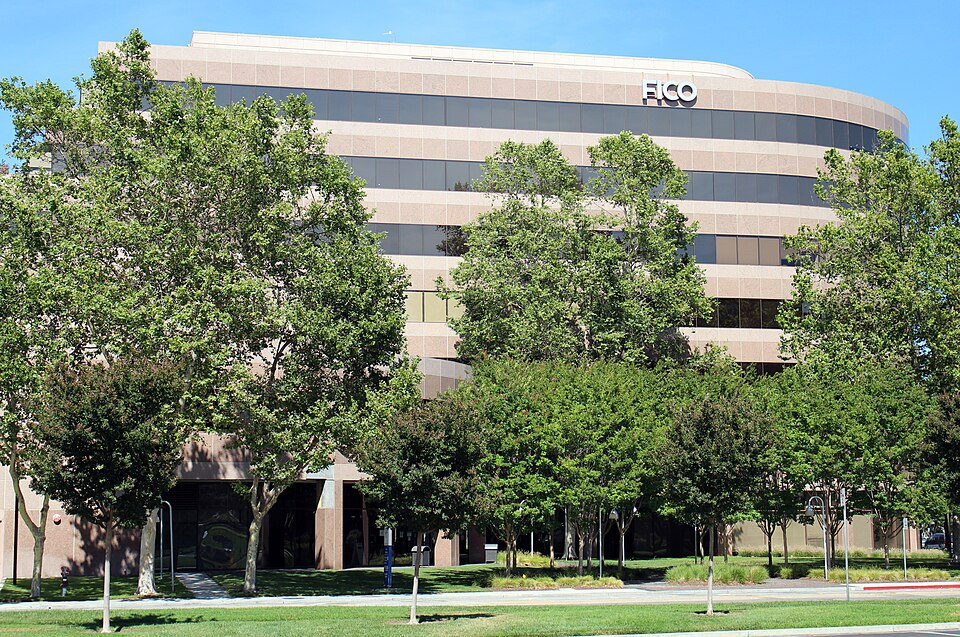
\includegraphics[height=0.40\textheight]{ch12_fico_hq_2020.jpg}\\[1mm]
\imgcap{FICO headquarters, San Jose, California}
\imgcredit{https://commons.wikimedia.org/wiki/File:Ficoheadquarters.jpg}{Photo: Coolcaesar (2020); CC BY-SA 4.0; Wikimedia Commons}
\end{column}
\end{columns}
\end{frame}

\begin{frame}{PD, LGD, EAD and the Expected Loss}
\itemsize{\small}
\begin{itemize}
    \item Three risk parameters of a loan (Basel II, \refBCBS)
    \begin{itemize}
        \item \textbf{PD}: probability of default within one year
        \item \textbf{LGD} (loss given default): the share of the exposure lost if default occurs, after recoveries
        \item \textbf{EAD} (exposure at default): the amount owed at the moment of default
    \end{itemize}
    \item \textbf{Expected loss}: $\mathrm{EL} = \mathrm{PD} \times \mathrm{LGD} \times \mathrm{EAD}$ (with independent PD and LGD)
    \begin{itemize}
        \item \textbf{Example}: a loan of 100\,000 RON with PD $= 2\%$, LGD $= 45\%$: EL $= 0.02 \times 0.45 \times 100\,000 = 900$ RON
        \item EL is a cost of doing business: it is priced into the interest rate and covered by provisions
    \end{itemize}
    \item Capital covers the \textbf{unexpected loss}: losses above EL in a bad year
\end{itemize}
\end{frame}

\begin{frame}{The Basel IRB Capital Formula}
\itemsize{\footnotesize}
\begin{columns}[T]
\begin{column}{0.62\textwidth}
\begin{itemize}
    \item \textbf{IRB} (internal ratings-based) approach: the bank estimates PD (and possibly LGD, EAD); the regulator gives the formula \refBCBS, ¶328--330
    \begin{itemize}
        \item $K = \mathrm{LGD}\left[\Phi\!\left(\dfrac{\Phi^{-1}(\mathrm{PD}) + \sqrt{R}\,\Phi^{-1}(0.999)}{\sqrt{1 - R}}\right) - \mathrm{PD}\right]$; RWA $= 12.5\,K\,$EAD
        \item $R$: the correlation of the borrowers with one common factor; RWA: risk-weighted assets, of which the bank holds at least 8\%
    \end{itemize}
    \item Logic \refGordy: the term in $\Phi(\cdot)$ is the PD in a year whose common factor is exceeded only with probability 0.1\%
    \begin{itemize}
        \item so $K$ is the credit VaR 0.1\% of the loss minus EL: the unexpected loss (\sfmchlink{https://danpele.github.io/SFM/EN/Courses/chapter10_var_es_backtesting.pdf}{Chapter 10})
    \end{itemize}
\end{itemize}
\end{column}
\begin{column}{0.34\textwidth}
\centering
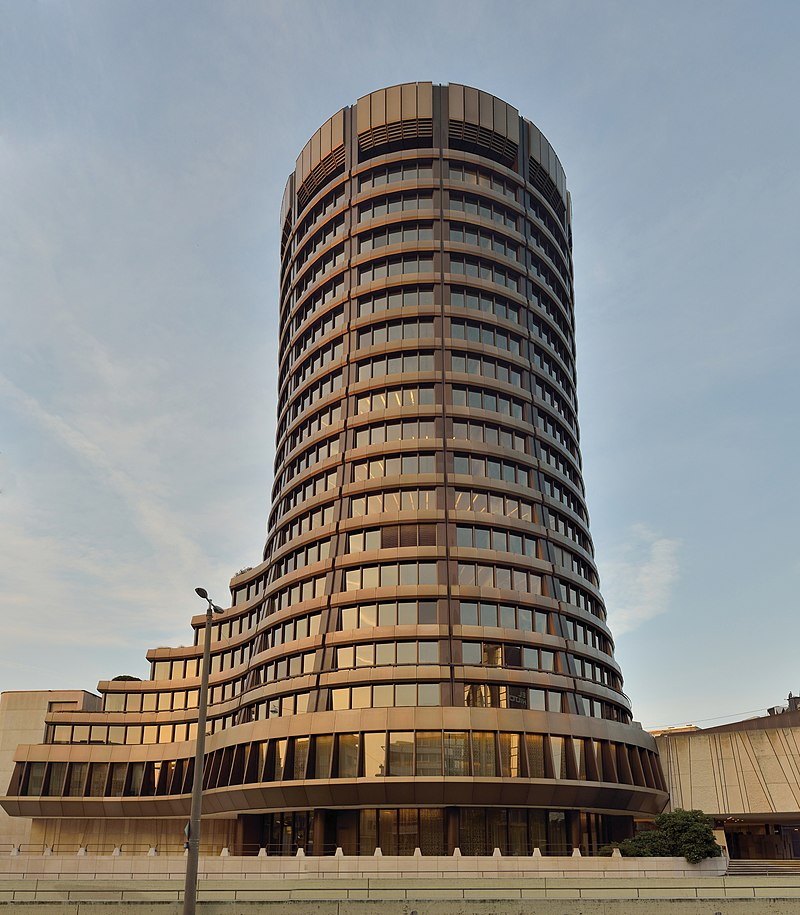
\includegraphics[height=0.40\textheight]{ch10_bis_tower_2014.jpg}\\[1mm]
\imgcap{The BIS tower in Basel}
\imgcredit{https://commons.wikimedia.org/wiki/File:Basel_Committee_on_Banking_Supervision_-_BCBS.jpg}{Photo: Taxiarchos228 (2014); CC BY-SA 4.0; Wikimedia Commons}
\end{column}
\end{columns}
\end{frame}

\begin{frame}{PD in Good and Bad Years: the One-Factor Model}
\itemsize{\footnotesize}
\begin{center}
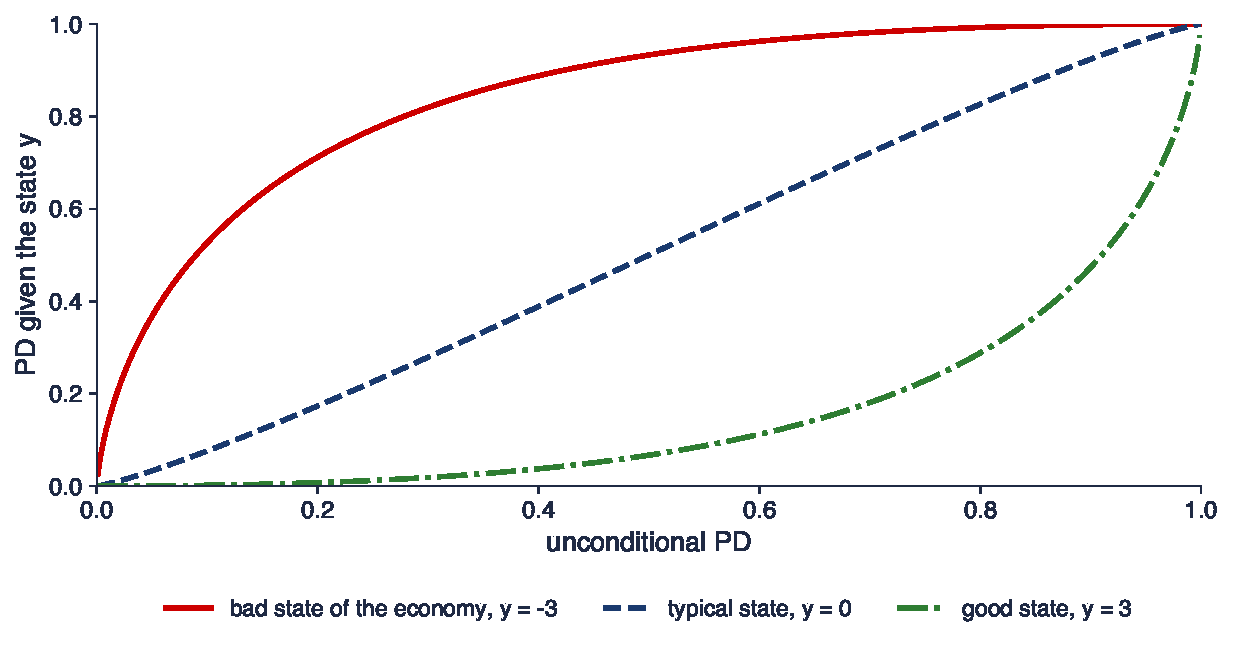
\includegraphics[width=0.97\textwidth,height=0.46\textheight,keepaspectratio]{sfm_ch12_conditional_pd.pdf}
\end{center}
\vspace{-0.25cm}
\begin{itemize}
    \item Borrower $i$ defaults if $\sqrt{\rho}\,Y + \sqrt{1 - \rho}\,\varepsilon_i < \Phi^{-1}(\mathrm{PD})$; $Y$: the state of the economy; given $Y = y$: PD$(y) = \Phi\big((\Phi^{-1}(\mathrm{PD}) - \sqrt{\rho}\,y)/\sqrt{1 - \rho}\big)$, $\rho = 0.2$
    \item Interpretation: a loan with PD $= 2\%$ defaults with probability 21.3\% in a bad year ($y = -3$), 1.1\% in a typical year and almost never in a good year; IRB uses $y = \Phi^{-1}(0.001)$
\end{itemize}
\sfmquantlet{Ch_12}{SFM_ch12_validation_irb}
\end{frame}

\begin{frame}{Worked Example: IRB Capital of a Retail Loan}
\itemsize{\footnotesize}
\begin{itemize}
    \item Other retail exposures: $R = 0.03\,w + 0.16\,(1 - w)$, $w = (1 - e^{-35\,\mathrm{PD}})/(1 - e^{-35})$ \refBCBS, ¶330
    \begin{itemize}
        \item PD $= 2\%$: $R = 0.095$; $\Phi^{-1}(0.02) = -2.054$, $\Phi^{-1}(0.999) = 3.090$
    \end{itemize}
    \item \textbf{Step by step}
    \begin{itemize}
        \item argument: $(-2.054 + \sqrt{0.095} \times 3.090)/\sqrt{1 - 0.095} = -1.160$; $\Phi(-1.160) = 12.31\%$: the PD in a bad year
        \item $K = 0.45 \times (12.31\% - 2\%) = 4.64\%$ of EAD: 4\,639 RON for a loan of 100\,000 RON
        \item RWA $= 12.5 \times 4\,639 = 57\,986$ RON: a risk weight of 58\%
    \end{itemize}
    \item Interpretation: EL ($900$ RON) is priced in; the capital ($4\,639$ RON) absorbs a year in which defaults reach 12.31\% instead of 2\%
\end{itemize}
\end{frame}

\begin{frame}{Expected Loss and IRB Capital as Functions of PD}
\itemsize{\footnotesize}
\begin{center}
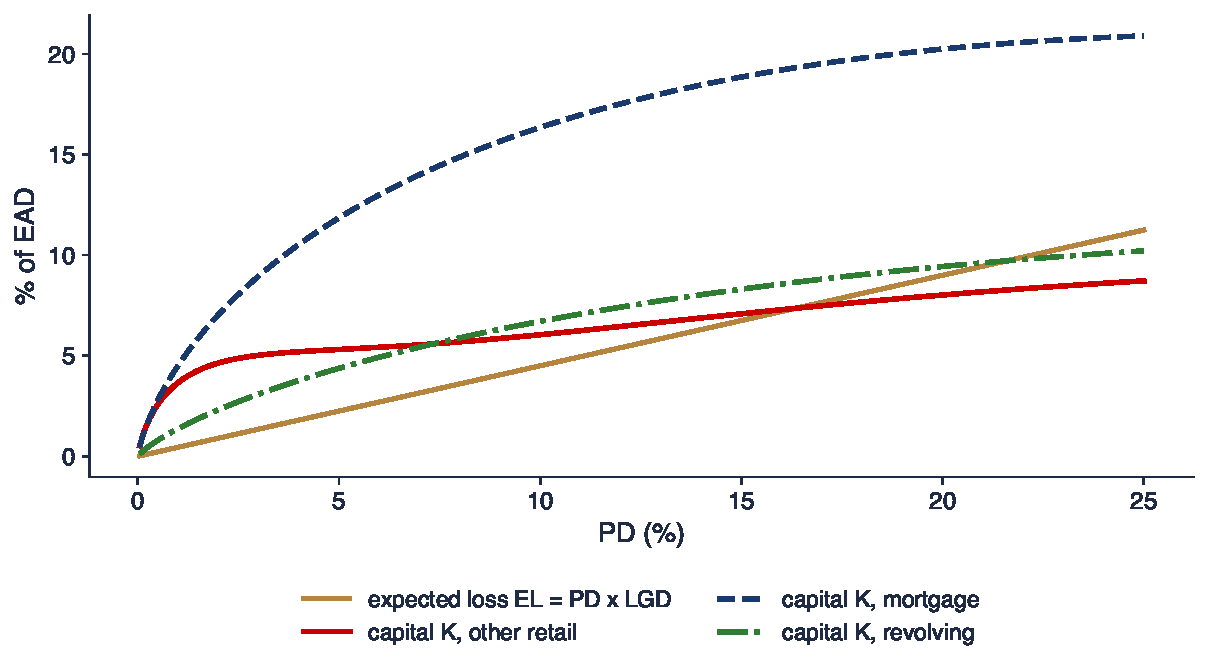
\includegraphics[width=0.97\textwidth,height=0.50\textheight,keepaspectratio]{sfm_ch12_irb.pdf}
\end{center}
\vspace{-0.25cm}
\begin{itemize}
    \item LGD $= 45\%$; capital $K$ for other retail ($R$ from 0.16 to 0.03), residential mortgages ($R = 0.15$) and revolving retail exposures ($R = 0.04$)
    \item Interpretation: EL grows linearly with PD; $K$ grows fast at low PD and then flattens, because a very risky loan is mostly an expected (priced) loss
\end{itemize}
\sfmquantlet{Ch_12}{SFM_ch12_validation_irb}
\end{frame}

\begin{frame}{Recap: What a Credit Score Is}
\itemsize{\small}
\begin{itemize}
    \item A score orders applicants by risk; a PD also gives the level of risk
    \item EL $=$ PD $\times$ LGD $\times$ EAD is priced in; Basel capital covers the unexpected loss (a credit VaR 0.1\% minus EL)
    \item Statistical scoring started with Fisher's discriminant analysis (Durand, 1941)
\end{itemize}
\end{frame}


%=============================================================================
\section{Default Data}
%=============================================================================

\begin{frame}{The South German Credit Data}
\itemsize{\small}
\begin{itemize}
    \item 1\,000 consumer credits of a large regional bank in southern Germany, 1973--1975 \refSGC; \refGroemping
    \begin{itemize}
        \item outcome: the contract was complied with (good) or not (bad, \textbf{default} $= 1$): 300 bad and 700 good credits
        \item 20 variables: checking account, duration, credit history, purpose, amount (DM, Deutsche Mark), savings, employment, age and others
    \end{itemize}
    \item A \textbf{stratified sample}: bad credits are heavily oversampled; the bad rate of the bank was about 5\% \refGroemping
    \begin{itemize}
        \item all borrowers had passed the bank's checks: rejected applicants are missing (reject inference, Section 8)
        \item the cost of accepting a bad credit is set to five times the cost of rejecting a good one
    \end{itemize}
    \item Licence CC BY 4.0; saved once in the course repository (data/credit)
\end{itemize}
\end{frame}

\begin{frame}{A Lesson in Data Checking}
\itemsize{\small}
\begin{itemize}
    \item The data were used for decades in the UCI version ``Statlog (German Credit)'', with code labels that were wrong \refGroemping
    \begin{itemize}
        \item in that version, ``no checking account'' was the safest group: 394 credits, 11.7\% bad
        \item in the corrected data, those 394 credits have a balance of at least 200 DM or a salary account; ``no checking account'' is the riskiest group (49.3\% bad)
    \end{itemize}
    \item The numbers were right, the labels were wrong: every model was fine, every interpretation of this variable was reversed
    \begin{itemize}
        \item checks: compare the frequency tables with the original source (here the book of Fahrmeir and Hamerle), ask whether the signs make economic sense
    \end{itemize}
    \item We use the corrected South German Credit data throughout
\end{itemize}
\end{frame}

\begin{frame}{Bad Rate by Checking Account}
\itemsize{\footnotesize}
\begin{center}
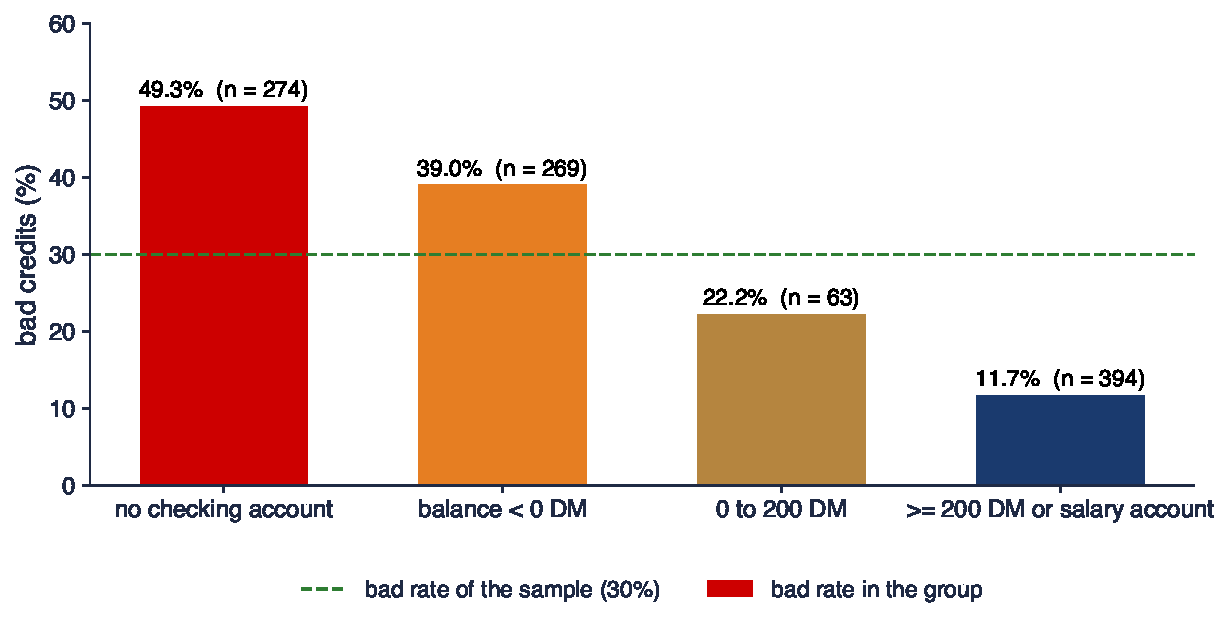
\includegraphics[width=0.97\textwidth,height=0.50\textheight,keepaspectratio]{sfm_ch12_default_by_status.pdf}
\end{center}
\vspace{-0.25cm}
\begin{itemize}
    \item Share of bad credits in each group; dashed: the sample average of 30\%
    \item Interpretation: the risk falls from 49.3\% (no account) to 11.7\% (balance of at least 200 DM): one variable already separates the applicants well
\end{itemize}
\sfmquantlet{Ch_12}{SFM_ch12_woe_iv}
\end{frame}

\begin{frame}{Class Imbalance and Oversampling}
\itemsize{\small}
\begin{itemize}
    \item Defaults are rare: a few percent of the loans of a bank; a sample with few bads tells little about them
    \begin{itemize}
        \item banks therefore oversample bads (here 30\% instead of about 5\%)
    \end{itemize}
    \item \textbf{Accuracy paradox}: the rule ``everybody is good'' is right for 70\% of this sample and for 77.9\% of the Taiwan data
    \begin{itemize}
        \item so accuracy alone is a poor measure; we need measures that look at the bads and the goods separately (Section 7)
    \end{itemize}
    \item \textbf{Taiwan credit card data} \refTW; \refYL: 30\,000 card holders, default on the October 2005 payment, 22.1\% defaults
    \begin{itemize}
        \item inputs: credit limit, age, the repayment status of April--September 2005, bills and payments; we use them for calibration and fairness
    \end{itemize}
\end{itemize}
\end{frame}

\begin{frame}{Training and Test Samples}
\itemsize{\small}
\begin{itemize}
    \item \textbf{Stratified split}: 700 credits for estimation (training), 300 for testing, with 30\% bads in both
    \begin{itemize}
        \item every choice (bins, WoE, variables, coefficients) is made on the training sample only
        \item the test sample is used once, at the end: it plays the role of the future applicants
    \end{itemize}
    \item \textbf{Leakage}: information from the test sample that enters the model, e.g.\ bins chosen on all data
    \begin{itemize}
        \item it makes the test result too optimistic; with 300 test credits one split is also noisy, so we add cross-validation (Section 7)
    \end{itemize}
\end{itemize}
\end{frame}

\begin{frame}{Recap: Default Data}
\itemsize{\small}
\begin{itemize}
    \item South German Credit: 1\,000 credits, 30\% bad by design; the widely used version had wrong labels
    \item Imbalance makes accuracy misleading; oversampling changes the level of PD, not the ranking
    \item Estimate on the training sample, judge on the test sample
\end{itemize}
\end{frame}


%=============================================================================
\section{Weight of Evidence and Information Value}
%=============================================================================

\begin{frame}{Weight of Evidence}
\itemsize{\footnotesize}
\begin{itemize}
    \item Split a variable into bins $i = 1, \dots, m$; $g_i$, $b_i$: goods and bads in bin $i$; $G$, $B$: their totals
    \begin{itemize}
        \item $\mathrm{WoE}_i = \ln\dfrac{g_i/G}{b_i/B}$: the log of the share of goods over the share of bads in the bin
    \end{itemize}
    \item Meaning: $\mathrm{WoE}_i = \ln\dfrac{g_i}{b_i} - \ln\dfrac{G}{B}$: the log-odds of being good in the bin minus the log-odds in the whole sample
    \begin{itemize}
        \item $\mathrm{WoE} > 0$: safer than average; $\mathrm{WoE} < 0$: riskier; $\mathrm{WoE} = 0$: no information
        \item a bin without goods or without bads would give $\pm\infty$: add 0.5 to both counts
    \end{itemize}
    \item \textbf{Information Value}: $\mathrm{IV} = \sum_i \left(\dfrac{g_i}{G} - \dfrac{b_i}{B}\right)\mathrm{WoE}_i \ge 0$
    \begin{itemize}
        \item a symmetric Kullback--Leibler divergence between the distributions of goods and bads across the bins
        \item rule of thumb \refSiddiqi: below 0.02 useless, 0.02--0.1 weak, 0.1--0.3 medium, above 0.3 strong
    \end{itemize}
\end{itemize}
\end{frame}

\begin{frame}{Worked Example: WoE and IV of the Checking Account}
\itemsize{\footnotesize}
\begin{center}
\scriptsize
\begin{tabular}{lrrrrrr}
\toprule
Checking account & goods & bads & $g_i/G$ & $b_i/B$ & WoE & IV term \\
\midrule
no checking account & 139 & 135 & $0.199$ & $0.450$ & $-0.818$ & $0.206$ \\
balance $<$ 0 DM & 164 & 105 & $0.234$ & $0.350$ & $-0.401$ & $0.046$ \\
0 to 200 DM & 49 & 14 & $0.070$ & $0.047$ & $0.405$ & $0.009$ \\
$\ge$ 200 DM or salary & 348 & 46 & $0.497$ & $0.153$ & $1.176$ & $0.404$ \\
total & 700 & 300 & 1 & 1 & & $0.666$ \\
\bottomrule
\end{tabular}
\end{center}
\begin{itemize}
    \item \textbf{Step by step}, last row: $g/G = 348/700 = 0.497$, $b/B = 46/300 = 0.153$
    \begin{itemize}
        \item WoE $= \ln(0.497/0.153) = 1.176$; IV term $= (0.497 - 0.153) \times 1.176 = 0.404$
    \end{itemize}
    \item Interpretation: IV $= 0.666 > 0.3$: a strong variable; the WoE falls monotonically from the safest to the riskiest group
\end{itemize}
\end{frame}

\begin{frame}{Binning: Rules of the Trade}
\itemsize{\small}
\begin{itemize}
    \item Why bins: they capture non-linear effects, limit the influence of outliers and give every applicant a small table of points
    \begin{itemize}
        \item numeric variables: a few intervals (here duration $\le 12$, 13--18, 19--24, 25--36, $> 36$ months); categorical: the categories
    \end{itemize}
    \item Rules \refSiddiqi; \refTCE
    \begin{itemize}
        \item at least about 5\% of the sample in every bin; merge small categories
        \item WoE should change in a way that makes economic sense (often monotonically)
        \item bins and WoE are estimated on the training sample and applied unchanged to new applicants
    \end{itemize}
    \item A WoE variable enters the logit with one coefficient: the scorecard stays additive and easy to read
\end{itemize}
\end{frame}

\begin{frame}{WoE of the Credit Duration}
\itemsize{\footnotesize}
\begin{center}
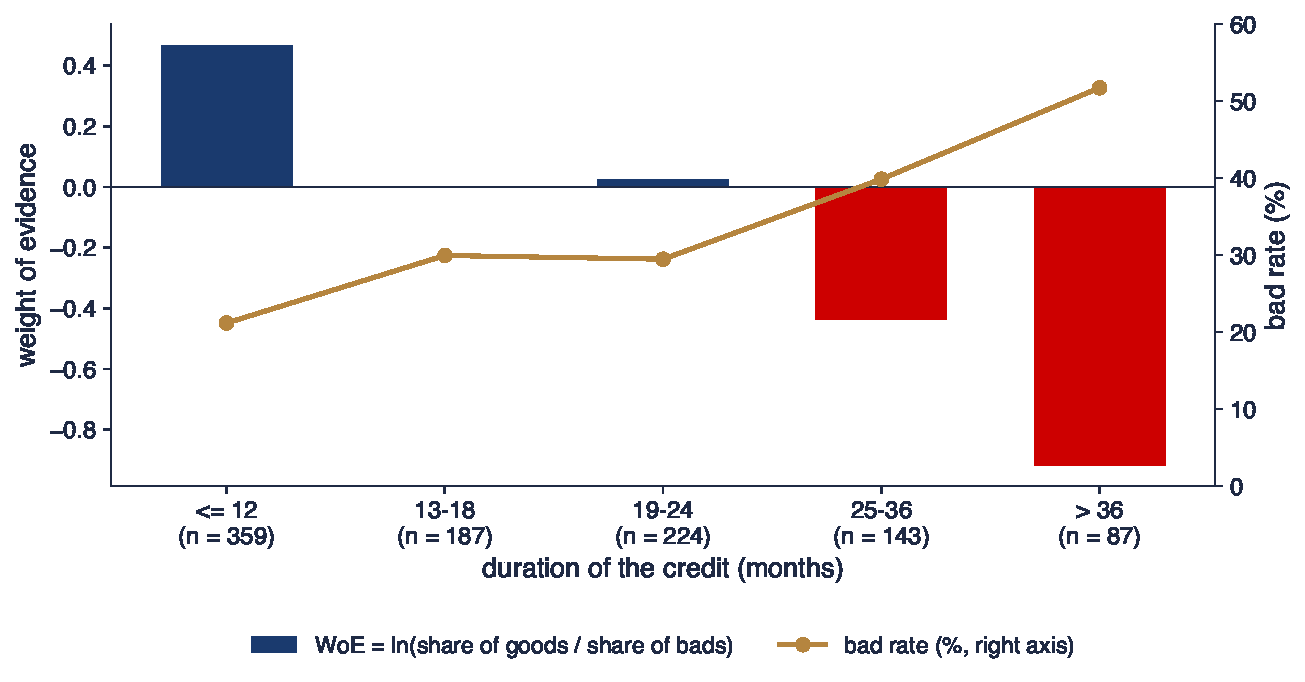
\includegraphics[width=0.97\textwidth,height=0.50\textheight,keepaspectratio]{sfm_ch12_woe_duration.pdf}
\end{center}
\vspace{-0.25cm}
\begin{itemize}
    \item Full sample; bars: WoE of each duration bin; line: bad rate (right axis); IV $= 0.182$ (medium)
    \item Interpretation: credits up to one year are safer (WoE $= 0.47$, 21\% bad); above three years the bad rate reaches 52\% (WoE $= -0.92$); 13--24 months are average
\end{itemize}
\sfmquantlet{Ch_12}{SFM_ch12_woe_iv}
\end{frame}

\begin{frame}{Information Value of the 20 Variables}
\itemsize{\footnotesize}
\begin{center}
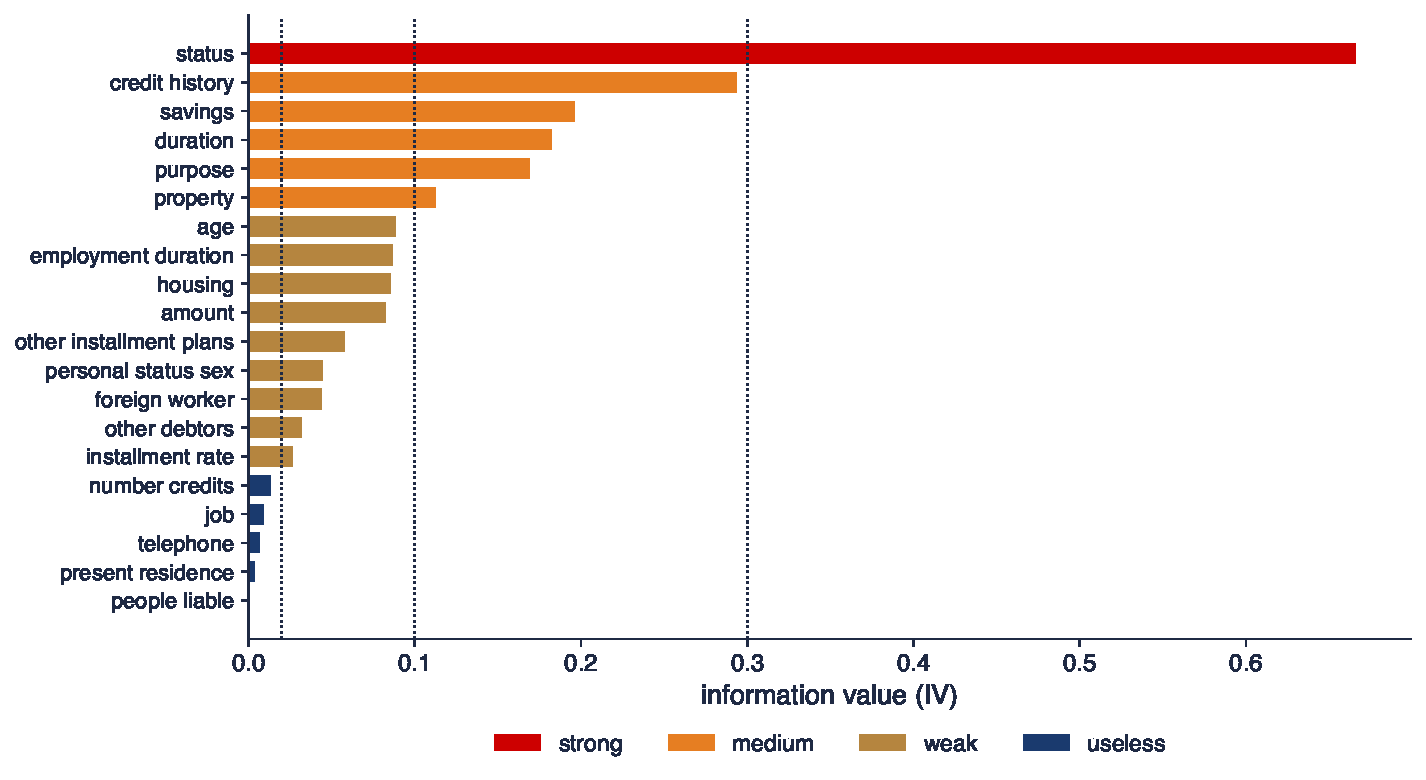
\includegraphics[width=0.97\textwidth,height=0.48\textheight,keepaspectratio]{sfm_ch12_iv.pdf}
\end{center}
\vspace{-0.25cm}
\begin{itemize}
    \item Full sample; dotted: the thresholds 0.02, 0.1 and 0.3; on the training sample, 6 variables have IV $\ge 0.1$ and enter the scorecard
    \item Interpretation: the checking account (IV $= 0.666$) and the credit history ($0.293$) dominate; telephone, residence and dependants carry no information
    \item IV looks at one variable at a time: two strong but correlated variables do not add their information
\end{itemize}
\sfmquantlet{Ch_12}{SFM_ch12_woe_iv}
\end{frame}

\begin{frame}{Recap: Weight of Evidence and Information Value}
\itemsize{\small}
\begin{itemize}
    \item WoE: log share of goods over share of bads in a bin; positive means safer than average
    \item IV ranks the variables; 0.1 and 0.3 mark medium and strong
    \item Bins, WoE and the selection of variables belong to the training sample
\end{itemize}
\end{frame}


%=============================================================================
\section{Logistic Regression}
%=============================================================================

\begin{frame}{Odds and Log-Odds}
\itemsize{\small}
\begin{itemize}
    \item A linear model $P(Y = 1) = \beta_0 + x^\top\beta$ can give probabilities below 0 or above 1
    \begin{itemize}
        \item we model a transformation of $p$ that can take any real value
    \end{itemize}
    \item \textbf{Odds} of default: $\dfrac{p}{1 - p} \in (0, \infty)$; \textbf{log-odds} (logit): $\ln\dfrac{p}{1 - p} \in (-\infty, \infty)$
    \begin{itemize}
        \item $p = 0.20$: odds $= 0.2/0.8 = 0.25$ (one default for four repaid loans); log-odds $= \ln 0.25 = -1.386$
        \item $p = 0.5$: odds 1, log-odds 0; the logit is symmetric: $\mathrm{logit}(1 - p) = -\mathrm{logit}(p)$
    \end{itemize}
    \item Bankers often speak of the \textbf{good:bad odds} $(1 - p)/p$: here 4:1
\end{itemize}
\end{frame}

\begin{frame}{The Logit Model}
\itemsize{\small}
\begin{itemize}
    \item $\ln\dfrac{p_i}{1 - p_i} = \beta_0 + x_i^\top\beta = \eta_i$, \quad $p_i = P(Y_i = 1 \mid x_i) = \dfrac{1}{1 + e^{-\eta_i}}$ \refCox
    \begin{itemize}
        \item $\beta_0$: the constant (intercept); $\eta_i$: the linear predictor, the log-odds of applicant $i$
    \end{itemize}
    \item \textbf{Maximum likelihood} (\sfmchlink{https://danpele.github.io/SFM/EN/Courses/chapter6_model_selection_risk_management.pdf}{Chapter 6}): $\ell(\beta) = \sum_i [y_i\ln p_i + (1 - y_i)\ln(1 - p_i)]$
    \begin{itemize}
        \item first-order condition $\sum_i (y_i - p_i)x_i = 0$: no closed form, solved by Newton--Raphson
        \item standard errors from the inverse of $\sum_i p_i(1 - p_i)x_ix_i^\top$; Wald test $z = \hat\beta_j/\mathrm{se}(\hat\beta_j)$
    \end{itemize}
    \item The logit is also used for corporate bankruptcy, starting with \refOhlson; the probit uses $\Phi(\eta)$ instead of the logistic function
    \begin{itemize}
        \item logit and probit give almost the same PDs; the logit has the odds interpretation
    \end{itemize}
\end{itemize}
\end{frame}

\begin{frame}{A Logistic Curve: PD and Duration}
\itemsize{\footnotesize}
\begin{center}
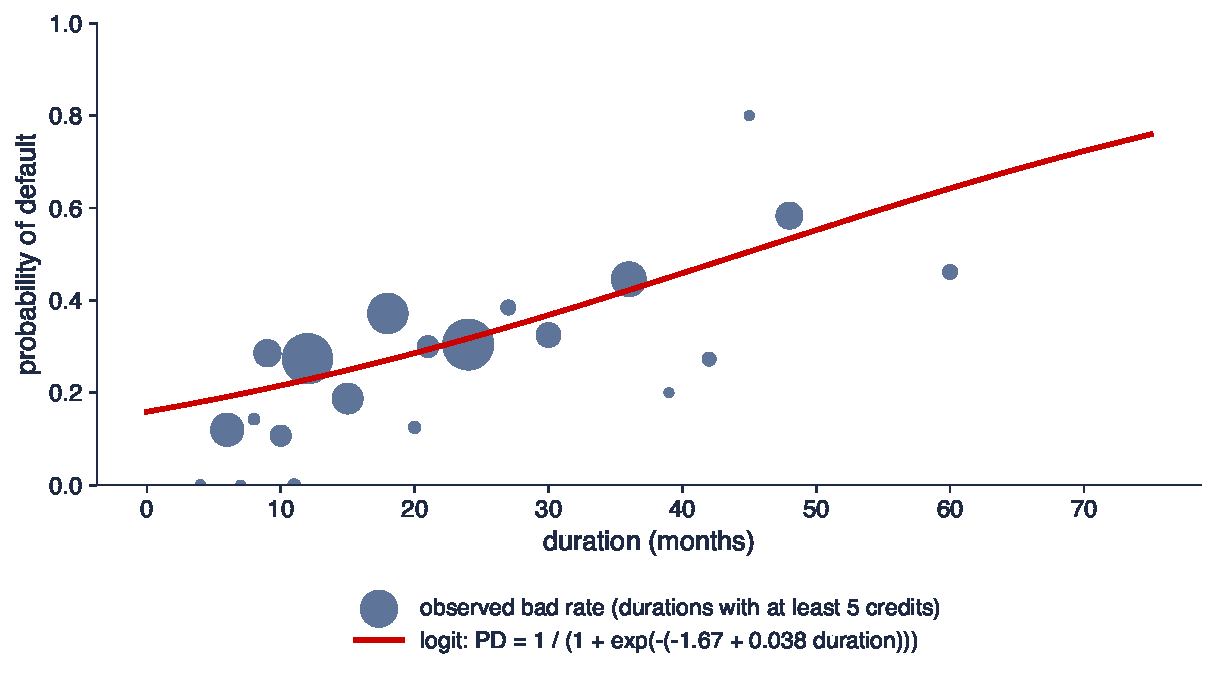
\includegraphics[width=0.97\textwidth,height=0.50\textheight,keepaspectratio]{sfm_ch12_logistic_curve.pdf}
\end{center}
\vspace{-0.25cm}
\begin{itemize}
    \item Logit with duration only: $\hat\beta_0 = -1.666$, $\hat\beta_1 = 0.0375$ per month (se $0.0057$); dots: observed bad rates
    \item Interpretation: each extra year multiplies the odds of default by $e^{12 \times 0.0375} = 1.57$; the PD rises from 22.9\% at 12 months to 53.4\% at 48 months
\end{itemize}
\sfmquantlet{Ch_12}{SFM_ch12_logit_lda}
\end{frame}

\begin{frame}{Interpreting the Coefficients}
\itemsize{\small}
\begin{itemize}
    \item $\beta_j$: the change in the \textbf{log-odds} when $x_j$ grows by one unit, the other variables fixed
    \begin{itemize}
        \item $e^{\beta_j}$: the \textbf{odds ratio}: the odds are multiplied by $e^{\beta_j}$; $100(e^{\beta_j} - 1)\%$ is the change in the odds
        \item a 95\% confidence interval: $\exp(\hat\beta_j \pm 1.96\,\mathrm{se})$
    \end{itemize}
    \item The effect on the \textbf{probability} depends on where the applicant is
    \begin{itemize}
        \item $\partial p/\partial x_j = p(1 - p)\beta_j$: largest at $p = 0.5$, small for very safe or very risky applicants
    \end{itemize}
    \item A dummy variable (0/1): $e^{\beta_j}$ compares the odds of the group with those of the reference group
    \begin{itemize}
        \item the interpretation needs a model that contains the relevant variables: an omitted variable changes the coefficients
    \end{itemize}
\end{itemize}
\end{frame}

\begin{frame}{A Small Logit on the Full Sample}
\itemsize{\footnotesize}
\begin{center}
\scriptsize
\begin{tabular}{lrrrrc}
\toprule
Variable & $\hat\beta$ & se & $z$ & p & odds ratio (95\% CI) \\
\midrule
constant & $-2.101$ & $0.311$ & $-6.75$ & $<$\,0.001 &  \\
duration (years) & $0.385$ & $0.092$ & $4.17$ & $<$\,0.001 & $1.47$ ($1.23$--$1.76$) \\
age (decades) & $-0.159$ & $0.069$ & $-2.30$ & 0.022 & $0.85$ ($0.74$--$0.98$) \\
amount (1000 DM) & $0.029$ & $0.032$ & $0.90$ & 0.368 & $1.03$ ($0.97$--$1.10$) \\
no checking account & $1.859$ & $0.188$ & $9.89$ & $<$\,0.001 & $6.42$ ($4.44$--$9.28$) \\
balance $<$ 0 DM & $1.338$ & $0.192$ & $6.99$ & $<$\,0.001 & $3.81$ ($2.62$--$5.55$) \\
\bottomrule
\end{tabular}
\end{center}
\begin{itemize}
    \item $n = 1\,000$; log-likelihood $-526.1$ against $-610.9$ with the constant only: LR $= 169.6$ on 5 degrees of freedom
    \item Reference group of the account dummies: a non-negative balance (0--200 DM, or at least 200 DM or a salary account)
\end{itemize}\sfmquantlet{Ch_12}{SFM_ch12_logit_lda}
\end{frame}

\begin{frame}{Odds Ratios with Confidence Intervals}
\itemsize{\footnotesize}
\begin{columns}[T]
\begin{column}{0.54\textwidth}
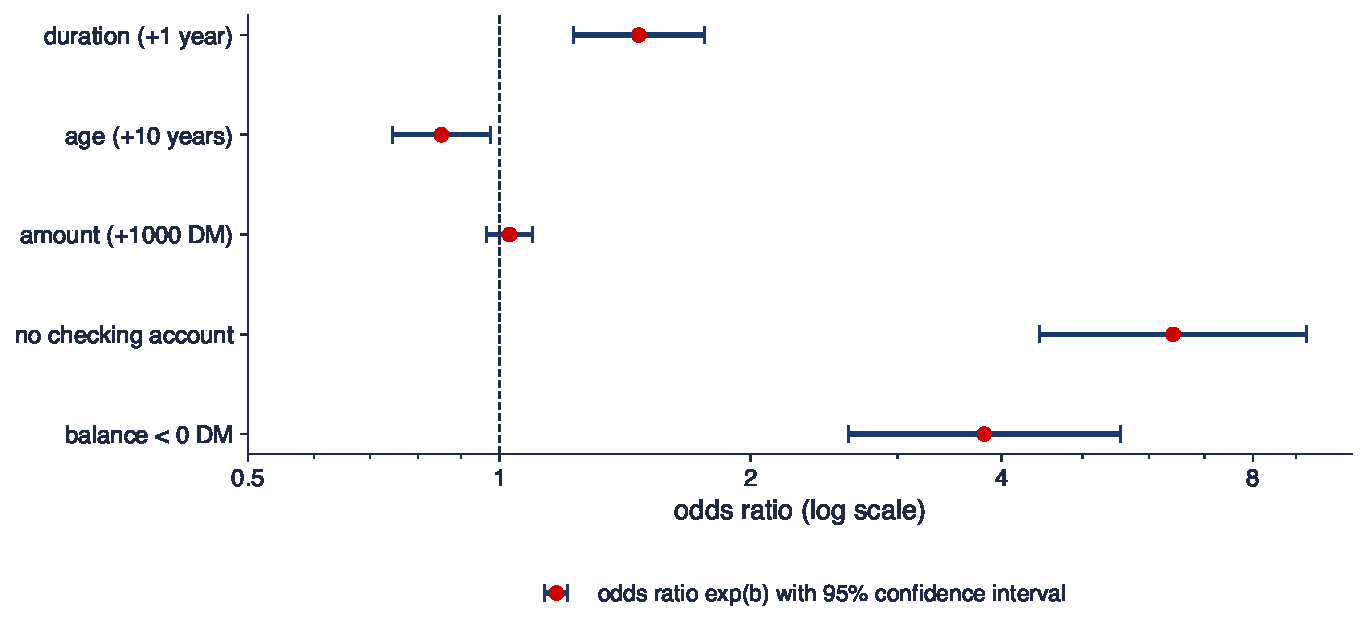
\includegraphics[width=\textwidth,height=0.55\textheight,keepaspectratio]{sfm_ch12_odds_ratios.pdf}
\end{column}
\begin{column}{0.44\textwidth}
\begin{itemize}
    \item Each dot: $e^{\hat\beta}$; bars: 95\% intervals; log scale; vertical line: no effect (1)
    \item Interpretation: without a checking account the odds of default are 6.42 times those of the reference group; a balance below zero multiplies them by 3.81
    \item One more year of duration raises the odds by 47\%; ten more years of age lower them by about 15\%
    \item The amount is not significant once the duration is in the model (the two are correlated)
\end{itemize}
\end{column}
\end{columns}
\sfmquantlet{Ch_12}{SFM_ch12_logit_lda}
\end{frame}

\begin{frame}{Worked Example: the PD of an Applicant}
\itemsize{\small}
\begin{itemize}
    \item Applicant: 36 months, 30 years old, 4000 DM, no checking account; coefficients of the previous table, rounded
    \begin{itemize}
        \item $\eta = -2.101 + 0.385 \times 3 + (-0.159) \times 3 + 0.029 \times 4 + 1.859$
        \item $\eta = -2.101 + 1.155 + (-0.477) + 0.116 + 1.859 = 0.552$
    \end{itemize}
    \item PD $= 1/(1 + e^{-0.552}) = 63.5\%$; odds $e^{0.552} = 1.74$
    \begin{itemize}
        \item the same applicant with a non-negative balance: $\eta = -1.307$, PD $= 21.3\%$
        \item one more year of duration: $\Delta p \approx p(1 - p)\beta \approx 8.9$ percentage points
    \end{itemize}
    \item Caution: this PD refers to a sample with 30\% bads, not to the bank's population (prior correction, two slides ahead)
\end{itemize}
\end{frame}

\begin{frame}{The WoE Logit Scorecard}
\itemsize{\footnotesize}
\begin{center}
\scriptsize
\begin{tabular}{lrrr}
\toprule
WoE variable & IV (training) & $\hat\beta$ & se \\
\midrule
constant & & $-0.850$ & $0.095$ \\
checking account & $0.591$ & $-0.829$ & $0.127$ \\
credit history & $0.215$ & $-0.675$ & $0.206$ \\
purpose & $0.205$ & $-0.937$ & $0.217$ \\
savings & $0.166$ & $-0.726$ & $0.246$ \\
duration & $0.159$ & $-1.082$ & $0.239$ \\
years with the employer & $0.122$ & $-0.873$ & $0.265$ \\
\bottomrule
\end{tabular}
\end{center}
\begin{itemize}
    \item Training sample (700 credits); each variable replaced by the WoE of its bin; logit for default
    \begin{itemize}
        \item all coefficients are negative: a higher WoE (safer bin) lowers the log-odds of default
        \item a coefficient of $-1$ would mean that the variable adds exactly its own WoE; values between $-0.7$ and $-1.1$ reflect the overlap between variables
    \end{itemize}
    \item Test sample: AUC $= 0.801$ (Section 7); in-sample log-likelihood $-347.2$
\end{itemize}\sfmquantlet{Ch_12}{SFM_ch12_scorecard}
\end{frame}

\begin{frame}{Correcting for Oversampling}
\itemsize{\small}
\begin{itemize}
    \item If bads and goods are sampled with different rates, only the constant of the logit changes
    \begin{itemize}
        \item $\ln\mathrm{odds}_{\text{pop}} = \ln\mathrm{odds}_{\text{sample}} + \ln\dfrac{\pi/(1 - \pi)}{\pi_s/(1 - \pi_s)}$; $\pi$: population bad rate, $\pi_s$: sample rate
        \item the slopes are unchanged: the ranking of the applicants does not depend on the sampling
    \end{itemize}
    \item \textbf{Step by step}: $\pi_s = 0.30$, $\pi = 0.05$: shift $= \ln(0.05/0.95) - \ln(0.30/0.70) = -2.944 - (-0.847) = -2.097$
    \begin{itemize}
        \item a sample PD of 30\% becomes 5\%; a sample PD of 50\% becomes 10.9\%
        \item the applicant of the worked example: $0.552 - 2.097 = -1.545$, PD $= 17.6\%$ in the bank's population instead of 63.5\%
    \end{itemize}
    \item Interpretation: AUC and Gini are unchanged by the correction; EL and capital are not
\end{itemize}
\end{frame}

\begin{frame}{Recap: Logistic Regression}
\itemsize{\small}
\begin{itemize}
    \item The logit models the log-odds linearly; $e^{\beta_j}$ is an odds ratio
    \item Estimated by maximum likelihood; the effect on PD is $p(1 - p)\beta_j$
    \item Oversampling moves only the constant: correct it before using PDs for EL or capital
\end{itemize}
\end{frame}


%=============================================================================
\section{Linear Discriminant Analysis}
%=============================================================================

\begin{frame}{Fisher's Idea (1936)}
\itemsize{\footnotesize}
\begin{columns}[T]
\begin{column}{0.55\textwidth}
\begin{itemize}
    \item \refFisher: find the linear combination $w^\top x$ that separates two groups best
    \begin{itemize}
        \item he used measurements of iris flowers; Durand applied it to loans five years later
    \end{itemize}
    \item Fisher criterion: $J(w) = \dfrac{[w^\top(m_1 - m_0)]^2}{w^\top S_W w}$
    \begin{itemize}
        \item $m_0$, $m_1$: mean vectors of goods and bads; $S_W$: the pooled within-group covariance matrix
        \item maximum: $w \propto S_W^{-1}(m_1 - m_0)$ \refMVA, Ch.~14
    \end{itemize}
    \item No distribution is needed for this criterion: it is a projection that maximises the distance between the groups relative to their spread
\end{itemize}
\end{column}
\begin{column}{0.43\textwidth}
\begin{columns}[T]
\begin{column}{0.48\textwidth}
\centering
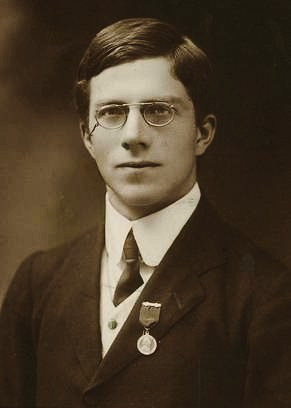
\includegraphics[height=0.34\textheight]{ch5_fisher_1913.jpg}\\[1mm]
\imgcap{R.A. Fisher, 1913}
\imgcredit{https://commons.wikimedia.org/wiki/File:Youngronaldfisher2.JPG}{Photo: unknown author (1913); public domain; Wikimedia Commons}
\end{column}
\begin{column}{0.48\textwidth}
\centering

\includegraphics[height=0.30\textheight]{ch12_iris_versicolor.jpg}\\[1mm]
\imgcap{Iris versicolor}
\imgcredit{https://commons.wikimedia.org/wiki/File:Iris_versicolor_-20200620-RM-100933.jpg}{Photo: Ermell (2020); CC BY-SA 4.0; Wikimedia Commons}
\end{column}
\end{columns}
\end{column}
\end{columns}
\end{frame}

\begin{frame}{LDA as a Probability Model}
\itemsize{\footnotesize}
\begin{itemize}
    \item Assume $x \mid Y = k \sim N(m_k, \Sigma)$, the same $\Sigma$ in both groups, and prior $\pi_1 = P(Y = 1)$
    \begin{itemize}
        \item Bayes: $\ln\dfrac{P(Y = 1 \mid x)}{P(Y = 0 \mid x)} = \underbrace{\ln\dfrac{\pi_1}{1 - \pi_1} - \tfrac12(m_1 + m_0)^\top w}_{c} + w^\top x$, \quad $w = \Sigma^{-1}(m_1 - m_0)$
        \item the log-odds are \textbf{linear in} $x$, exactly as in the logit; the prior enters only the constant
    \end{itemize}
    \item The difference is in the estimation
    \begin{itemize}
        \item LDA: plug in the sample means and the pooled covariance (a closed form)
        \item logit: maximise the conditional likelihood of $Y$ given $x$; no assumption on the distribution of $x$
    \end{itemize}
    \item Classification rule: assign to ``bad'' if $c + w^\top x > \ln(C_{FP}/C_{FN})$ (costs, Section 7)
\end{itemize}
\end{frame}

\begin{frame}{Worked Example: Fisher's Direction with Two Variables}
\itemsize{\footnotesize}
\begin{itemize}
    \item $x = $ (duration in months, age in years), full sample: 700 goods, 300 bads
    \begin{itemize}
        \item $m_0 = (19.21, 36.22)$, $m_1 = (24.86, 33.96)$, $m_1 - m_0 = (5.65, -2.26)$
        \item $S_W = \begin{pmatrix} 138.8 & -2.46 \\ -2.46 & 127.9 \end{pmatrix}$, $\det S_W = 17756$
    \end{itemize}
    \item \textbf{Step by step}: $S_W^{-1} = \dfrac{1}{\det S_W}\begin{pmatrix} 127.9 & -(-2.46) \\ -(-2.46) & 138.8 \end{pmatrix}$, $w = S_W^{-1}(m_1 - m_0) = (0.0404, -0.0169)$
    \begin{itemize}
        \item logit with the same two variables: slopes $(0.0375, -0.0183)$
        \item ratio duration/age: LDA $-2.39$, logit $-2.05$: one month of duration weighs as much as about two years of age, in the other direction
    \end{itemize}
\end{itemize}
\end{frame}

\begin{frame}{Fisher's Boundary and the Logit Boundary}
\itemsize{\footnotesize}
\begin{center}
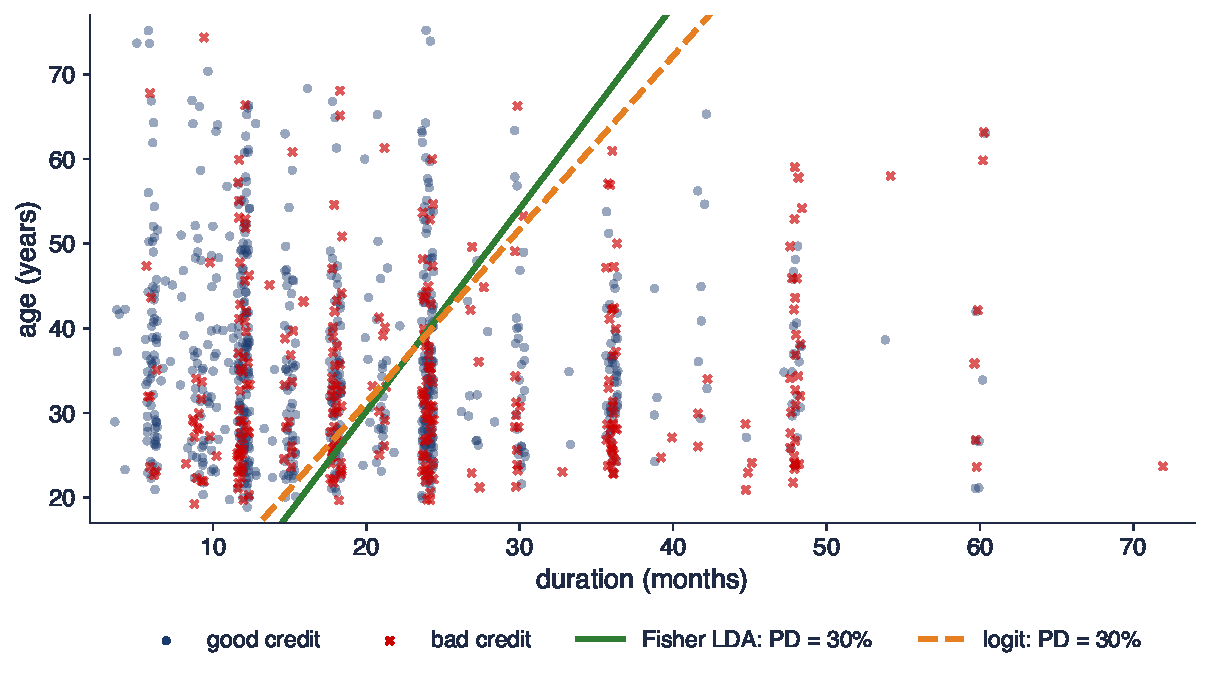
\includegraphics[width=0.97\textwidth,height=0.50\textheight,keepaspectratio]{sfm_ch12_lda_2d.pdf}
\end{center}
\vspace{-0.25cm}
\begin{itemize}
    \item Duration and age of every credit (a small jitter added); lines: the points with PD $= 30\%$ (the sample rate) for the LDA and for the logit
    \item Interpretation: both boundaries are lines with almost the same slope; the two clouds overlap heavily, so two variables are far from enough
\end{itemize}
\sfmquantlet{Ch_12}{SFM_ch12_logit_lda}
\end{frame}

\begin{frame}{Logit or LDA?}
\itemsize{\footnotesize}
\begin{center}
\scriptsize
\begin{tabular}{p{3.0cm}p{3.9cm}p{3.9cm}}
\toprule
& \textbf{Logit} & \textbf{LDA (Fisher)} \\
\midrule
model & $P(Y \mid x)$ only & $P(x \mid Y)$ Normal, common $\Sigma$ \\
estimation & maximum likelihood, iterative & means and covariance, closed form \\
if $x$ is Normal & consistent, less efficient & more efficient \\
dummies, WoE, skewed $x$ & fine & ranking fine, PDs may be off \\
test AUC (WoE inputs) & $0.801$ & $0.801$ \\
\bottomrule
\end{tabular}
\end{center}
\begin{itemize}
    \item Test sample: the correlation of the two log-odds scores is $0.999$; DeLong test of equal AUCs: $z = 0.18$, p $= 0.86$ \refDeLong
    \item Interpretation: for ranking, the two methods are practically identical; the logit is preferred for PDs because it does not need Normal inputs
\end{itemize}\sfmquantlet{Ch_12}{SFM_ch12_logit_lda}
\end{frame}

\begin{frame}{Recap: Linear Discriminant Analysis}
\itemsize{\small}
\begin{itemize}
    \item Fisher: $w \propto S_W^{-1}(m_1 - m_0)$ maximises the separation of the groups
    \item With Normal classes and a common covariance, LDA has linear log-odds, like the logit
    \item On our data both rank equally well; the logit gives more reliable PDs
\end{itemize}
\end{frame}


%=============================================================================
\section{From Model to Scorecard}
%=============================================================================

\begin{frame}{Scaling a Scorecard}
\itemsize{\small}
\begin{itemize}
    \item \textbf{Scorecard}: a table that gives points to every attribute; the score of an applicant is the sum of the points \refSiddiqi
    \begin{itemize}
        \item higher score $=$ lower risk; the score is a linear function of the good:bad log-odds
    \end{itemize}
    \item $\text{Score} = \text{Offset} + \text{Factor} \times \ln\dfrac{1 - p}{p}$, two conventions fix the scale
    \begin{itemize}
        \item \textbf{PDO} (points to double the odds): $+$PDO points $\Leftrightarrow$ the good:bad odds double: Factor $=$ PDO$/\ln 2$
        \item a base score at given odds: Offset $=$ Base $-$ Factor $\ln(\text{odds}_0)$
    \end{itemize}
    \item Here: PDO $= 20$, 600 points at odds 50:1
    \begin{itemize}
        \item Factor $= 20/\ln 2 = 28.85$; Offset $= 600 - 28.85 \times \ln 50 = 600 - 28.85 \times 3.912 = 487.12$
    \end{itemize}
\end{itemize}
\end{frame}

\begin{frame}{Worked Example: Scores and Points}
\itemsize{\footnotesize}
\begin{itemize}
    \item \textbf{PD to score}: PD $= 5\%$, odds 19:1: Score $= 487.12 + 28.85 \times \ln 19 = 487.12 + 28.85 \times 2.944 = 572.1$
    \begin{itemize}
        \item PD $= 30\%$ (odds 7:3): $487.12 + 28.85 \times 0.847 = 511.6$
    \end{itemize}
    \item \textbf{Score to PD}: 560 points: $\ln$ odds $= (560 - 487.12)/28.85 = 2.526$, odds $12.5$:1, PD $= 7.4\%$
    \item \textbf{Points of an attribute} ($k = 6$ variables; logit for default with constant $\beta_0$ and slope $\beta_j$)
    \begin{itemize}
        \item $\text{points}_{ij} = -(\beta_j\,\mathrm{WoE}_{ij} + \beta_0/k)\,\text{Factor} + \text{Offset}/k$; the minus sign turns default log-odds into good:bad log-odds
        \item checking account (training WoE): no account 66 points, balance $<$ 0 77, 0--200 DM 97, at least 200 DM or salary 110
    \end{itemize}
    \item Prior correction in points: for a population with 5\% bads the default log-odds fall by $2.097$, so the good:bad log-odds rise by $2.097$ and every score rises by $28.85 \times 2.097 = 60.5$ points
\end{itemize}\sfmquantlet{Ch_12}{SFM_ch12_scorecard}
\end{frame}

\begin{frame}{Scores of the Test Sample}
\itemsize{\footnotesize}
\begin{center}
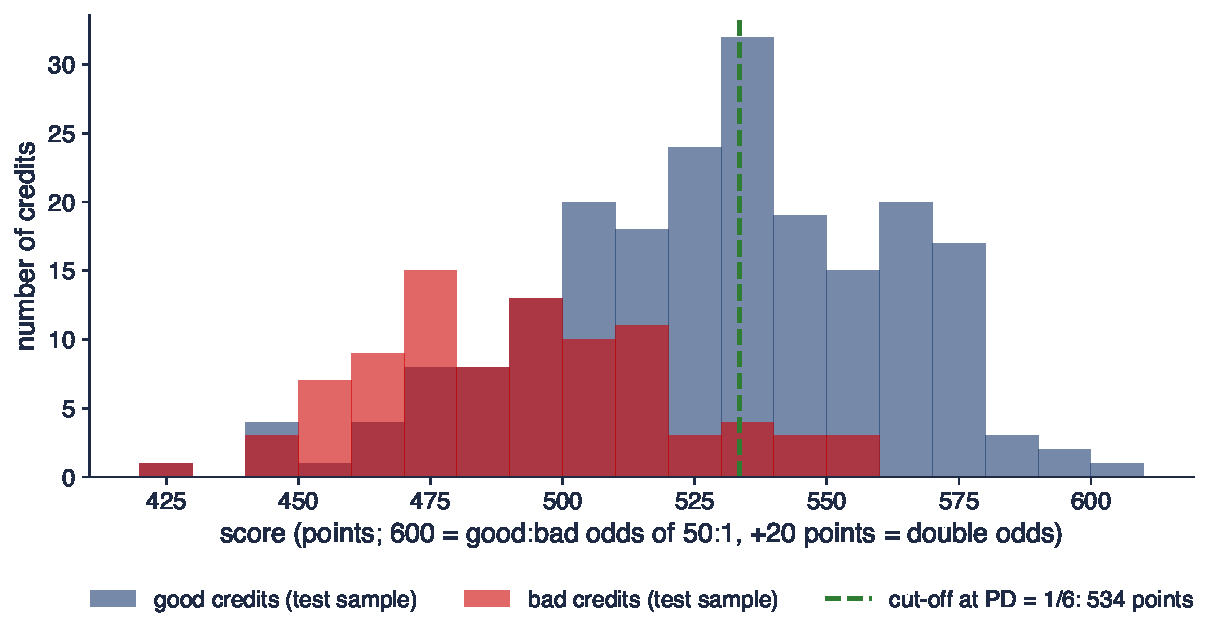
\includegraphics[width=0.97\textwidth,height=0.50\textheight,keepaspectratio]{sfm_ch12_score_dist.pdf}
\end{center}
\vspace{-0.25cm}
\begin{itemize}
    \item 300 test credits; scores from 422 to 607 points; mean: goods 529, bads 492; dashed: the cut-off at PD $= 1/6$ (Section 7), 534 points
    \item Interpretation: the two distributions are shifted but overlap: every cut-off rejects some goods and accepts some bads; the validation measures quantify this overlap
\end{itemize}
\sfmquantlet{Ch_12}{SFM_ch12_scorecard}
\end{frame}


%=============================================================================
\section{Validation}
%=============================================================================

\begin{frame}{The Confusion Matrix}
\itemsize{\footnotesize}
\begin{columns}[T]
\begin{column}{0.50\textwidth}
\begin{center}
\scriptsize
\begin{tabular}{lcc}
\toprule
& predicted bad (reject) & predicted good (accept) \\
\midrule
actual bad & TP & FN \\
actual good & FP & TN \\
\bottomrule
\end{tabular}
\end{center}

\end{column}
\begin{column}{0.48\textwidth}
\begin{itemize}
    \item A cut-off $c$: reject if PD $> c$
    \item TP (true positive): a bad rejected; FN (false negative): a bad accepted
    \item FP (false positive): a good rejected; TN (true negative): a good accepted
\end{itemize}
\end{column}
\end{columns}\begin{itemize}
    \item Rates
    \begin{itemize}
        \item \textbf{TPR} (true positive rate, sensitivity) $= \mathrm{TP}/(\mathrm{TP} + \mathrm{FN})$: share of bads caught
        \item \textbf{FPR} (false positive rate) $= \mathrm{FP}/(\mathrm{FP} + \mathrm{TN}) = 1 -$ specificity: share of goods rejected
        \item precision $= \mathrm{TP}/(\mathrm{TP} + \mathrm{FP})$; accuracy $= (\mathrm{TP} + \mathrm{TN})/n$
    \end{itemize}
    \item Every rate depends on $c$; the measures that follow summarise all cut-offs at once
\end{itemize}
\end{frame}

\begin{frame}{Two Cut-Offs on the Test Sample}
\itemsize{\footnotesize}
\begin{center}
\scriptsize
\begin{tabular}{lrrrrrrrr}
\toprule
cut-off & TP & FN & FP & TN & accuracy & TPR & FPR & cost \\
\midrule
PD $> 0.5$ & 43 & 47 & 25 & 185 & $76.0\%$ & $47.8\%$ & $11.9\%$ & $0.867$ \\
PD $> 1/6$ & 82 & 8 & 112 & 98 & $60.0\%$ & $91.1\%$ & $53.3\%$ & $0.507$ \\
\bottomrule
\end{tabular}
\end{center}
\begin{itemize}
    \item Cost per applicant $= (5\,\mathrm{FN} + 1\,\mathrm{FP})/n$: accepting a bad costs five times as much as rejecting a good \refGroemping
    \begin{itemize}
        \item the Bayes cut-off minimises the expected cost: reject if $p\,C_{FN} > (1 - p)\,C_{FP}$, i.e.\ $p > C_{FP}/(C_{FP} + C_{FN}) = 1/6$
    \end{itemize}
    \item Interpretation: the cut-off of 1/6 has a lower accuracy (60.0\% against 76.0\%) but a much lower cost (0.507 against 0.867): it catches 91.1\% of the bads
\end{itemize}\sfmquantlet{Ch_12}{SFM_ch12_validation_irb}
\end{frame}

\begin{frame}{Expected Cost and the Choice of the Cut-Off}
\itemsize{\footnotesize}
\begin{center}
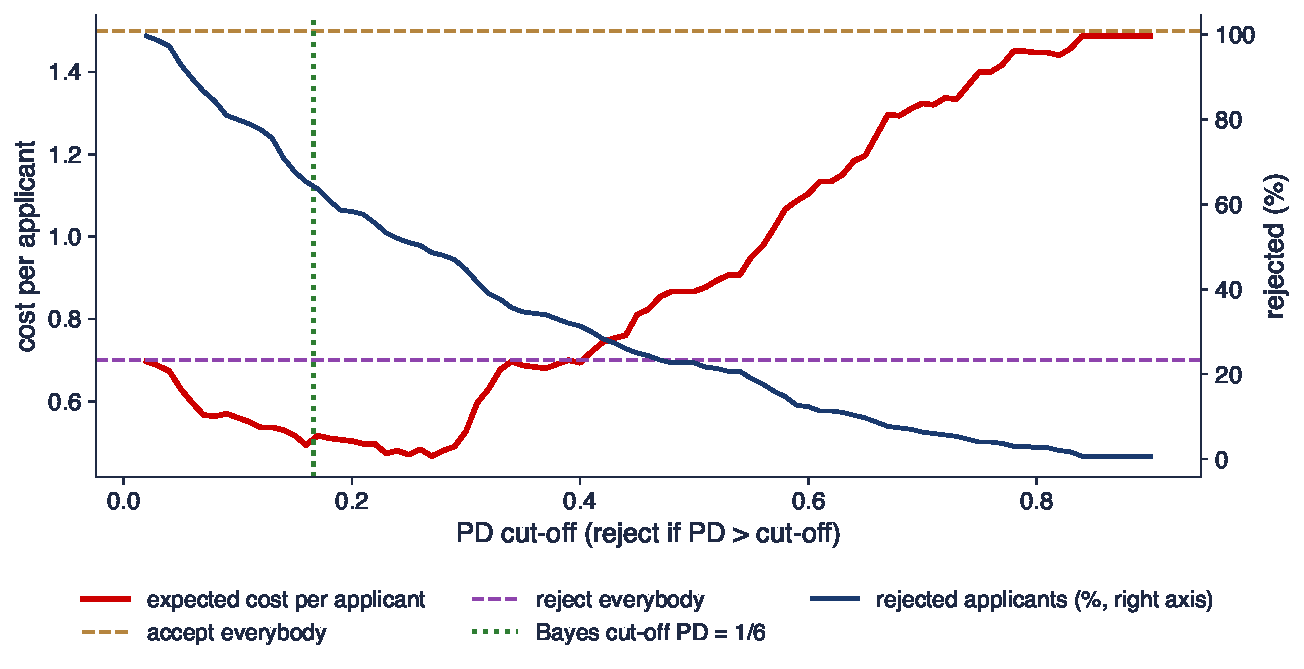
\includegraphics[width=0.97\textwidth,height=0.50\textheight,keepaspectratio]{sfm_ch12_cost_cutoff.pdf}
\end{center}
\vspace{-0.25cm}
\begin{itemize}
    \item Test sample; red: cost per applicant; dashed: accept everybody (1.50) or reject everybody (0.70); blue: share rejected (right axis)
    \item Interpretation: the cost is flat between PD 0.1 and 0.3; the minimum on these 300 credits is at 0.27, close to the Bayes cut-off of 1/6, which is chosen before seeing the test data
\end{itemize}
\sfmquantlet{Ch_12}{SFM_ch12_validation_irb}
\end{frame}

\begin{frame}{ROC Curve and AUC}
\itemsize{\small}
\begin{itemize}
    \item \textbf{ROC} (receiver operating characteristic): the points (FPR$(c)$, TPR$(c)$) for all cut-offs $c$
    \begin{itemize}
        \item from (0, 0) (reject nobody) to (1, 1) (reject everybody); the diagonal is a random score
    \end{itemize}
    \item \textbf{AUC} (area under the curve) $= P(s_{\text{bad}} > s_{\text{good}}) + \tfrac12 P(s_{\text{bad}} = s_{\text{good}})$ \refHM
    \begin{itemize}
        \item $s$: the risk score (here the PD); compute it by counting pairs: the share of (bad, good) pairs ordered correctly
        \item the Mann--Whitney statistic divided by $n_1 n_0$; 0.5: no discrimination, 1: perfect
    \end{itemize}
    \item \textbf{Gini} $= 2\,\mathrm{AUC} - 1$; AUC does not depend on the bad rate or on a monotone rescaling of the score
    \begin{itemize}
        \item standard error and tests of AUC: \refDeLong
    \end{itemize}
\end{itemize}
\end{frame}

\begin{frame}{ROC Curves on the Test Sample}
\itemsize{\footnotesize}
\begin{columns}[T]
\begin{column}{0.47\textwidth}
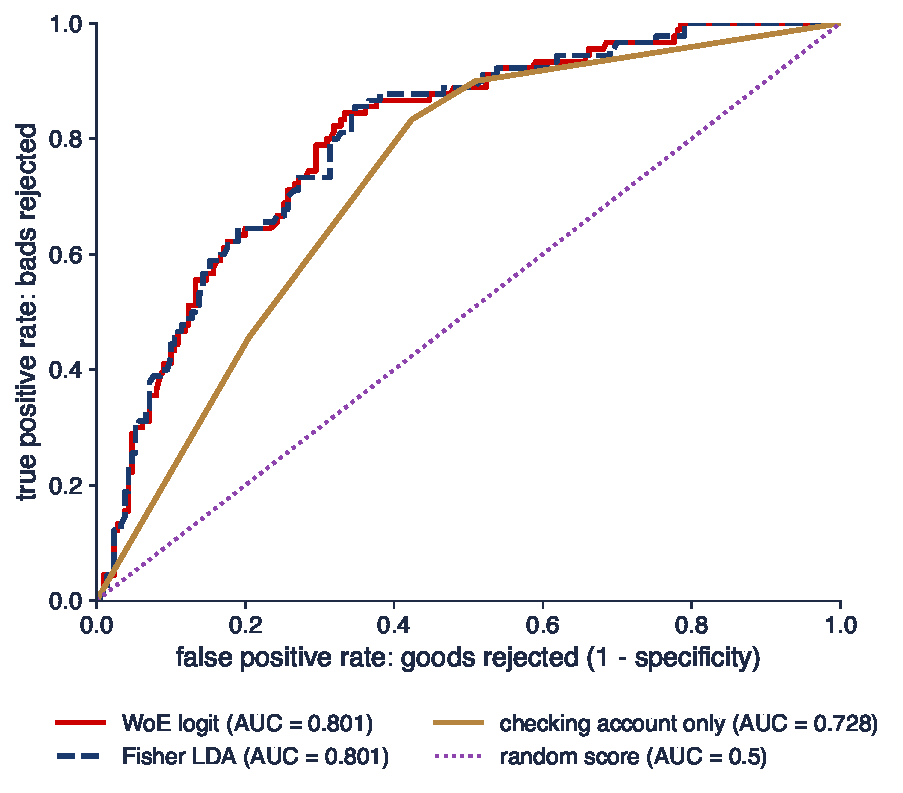
\includegraphics[width=\textwidth,height=0.64\textheight,keepaspectratio]{sfm_ch12_roc.pdf}
\end{column}
\begin{column}{0.51\textwidth}
\begin{itemize}
    \item 300 test credits, 18\,900 (bad, good) pairs
    \item WoE logit: AUC $= 0.801$, 95\% CI $[0.749, 0.854]$ (DeLong, se $0.027$); Gini $= 0.603$
    \item Checking account alone: AUC $= 0.728$; DeLong test against the scorecard: $z = 2.86$, p $= 0.004$
    \item Interpretation: a random bad has a higher PD than a random good in about 80\% of the pairs; the other five variables add a significant improvement over the checking account
\end{itemize}
\end{column}
\end{columns}
\sfmquantlet{Ch_12}{SFM_ch12_validation_irb}
\end{frame}

\begin{frame}{CAP Curve, Accuracy Ratio and KS}
\itemsize{\small}
\begin{itemize}
    \item \textbf{CAP} (cumulative accuracy profile): sort the applicants from the riskiest; plot the share of all bads among the first $x\%$
    \begin{itemize}
        \item perfect model: all bads first, the curve reaches 1 at $x = $ bad rate; random: the diagonal
        \item \textbf{AR} (accuracy ratio) $= \dfrac{\text{area between model CAP and diagonal}}{\text{area between perfect CAP and diagonal}}$; for a continuous score AR $=$ Gini
    \end{itemize}
    \item \textbf{KS} (Kolmogorov--Smirnov): $\max_s |F_{\text{bad}}(s) - F_{\text{good}}(s)|$, the largest gap between the score distributions of bads and goods
    \begin{itemize}
        \item read on the ROC curve: KS $= \max_c\,(\mathrm{TPR} - \mathrm{FPR})$; the score where it occurs is a natural first cut-off
    \end{itemize}
    \item All three measure \textbf{discrimination} (ranking), not calibration
\end{itemize}
\end{frame}

\begin{frame}{CAP and KS on the Test Sample}
\itemsize{\footnotesize}
\begin{columns}[T]
\begin{column}{0.44\textwidth}
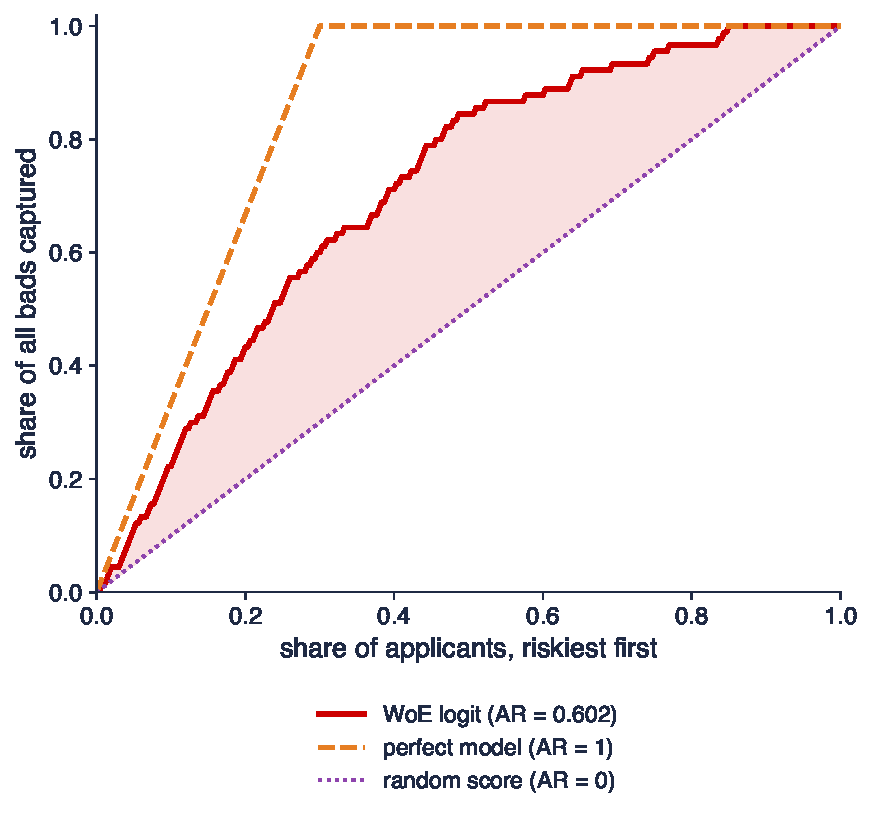
\includegraphics[width=\textwidth,height=0.50\textheight,keepaspectratio]{sfm_ch12_cap.pdf}
\end{column}
\begin{column}{0.54\textwidth}
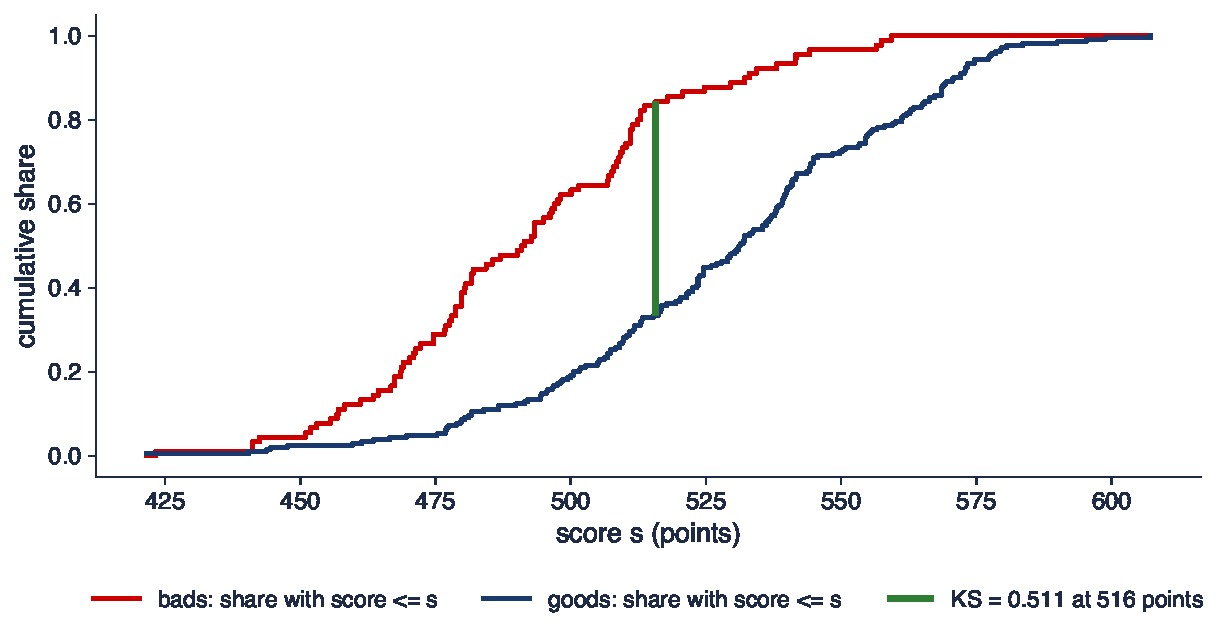
\includegraphics[width=\textwidth,height=0.50\textheight,keepaspectratio]{sfm_ch12_ks.pdf}
\end{column}
\end{columns}\begin{itemize}
    \item AR $= 0.602$ (Gini $= 0.603$: the same up to rounding); KS $= 0.511$ at 516 points
    \item Interpretation: rejecting the riskiest 30\% catches about two thirds of the bads; at 516 points the scorecard separates bads and goods best
\end{itemize}\sfmquantlet{Ch_12}{SFM_ch12_validation_irb}
\end{frame}

\begin{frame}{Calibration and the Brier Score}
\itemsize{\small}
\begin{itemize}
    \item \textbf{Calibration}: among applicants with PD $\approx p$, a share of about $p$ defaults
    \begin{itemize}
        \item reliability diagram: sort by PD, form groups (e.g.\ ten), plot the mean PD against the observed default rate
        \item Hosmer--Lemeshow \refHL: $\sum_g \dfrac{(O_g - n_g\bar p_g)^2}{n_g\bar p_g(1 - \bar p_g)} \approx \chi^2(G - 2)$
    \end{itemize}
    \item \textbf{Brier score} \refBrier: $\mathrm{BS} = \frac1n\sum_i (p_i - y_i)^2$, the mean squared error of the PDs; lower is better
    \begin{itemize}
        \item reference: a constant PD equal to the training bad rate; skill $= 1 - \mathrm{BS}/\mathrm{BS}_{\text{ref}}$
        \item scorecard test sample: BS $= 0.162$ against $0.210$ (skill 23\%); HL with 10 groups $= 6.520$, p $= 0.589$
    \end{itemize}
    \item Brier rewards both ranking and calibration; AUC sees only the ranking
\end{itemize}
\end{frame}

\begin{frame}{Calibration on the Taiwan Data}
\itemsize{\footnotesize}
\begin{columns}[T]
\begin{column}{0.44\textwidth}
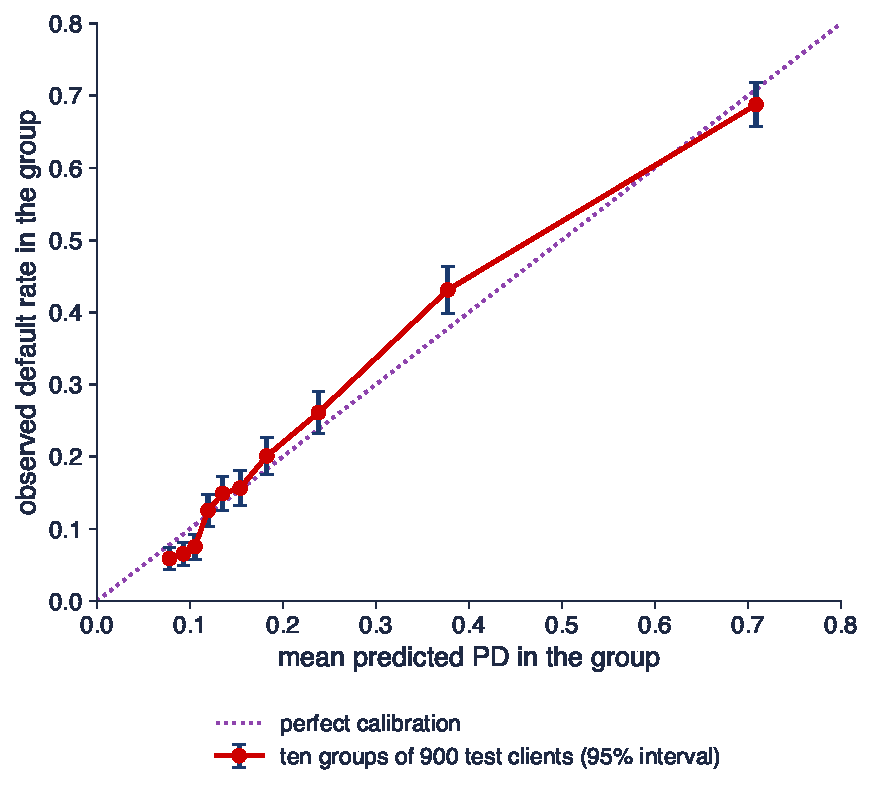
\includegraphics[width=\textwidth,height=0.62\textheight,keepaspectratio]{sfm_ch12_calibration.pdf}
\end{column}
\begin{column}{0.54\textwidth}
\begin{itemize}
    \item Logit on 30\,000 card holders (70\% estimation); test sample of 9\,000; ten groups of 900 by PD; bars: 95\% intervals
    \item Test AUC $= 0.777$ (estimation $0.774$); Brier $= 0.136$ against $0.172$ (skill 21\%)
    \item Hosmer--Lemeshow $= 40.660$, p $<$\,0.001: rejected, although the points lie close to the diagonal
    \item Interpretation: with 9000 clients the test detects small deviations (the safest group: PD 7.8\%, observed 5.9\%); judge the size of the gaps, not only the p-value
\end{itemize}
\end{column}
\end{columns}
\sfmquantlet{Ch_12}{SFM_ch12_validation_irb}
\end{frame}

\begin{frame}{Out-of-Sample and Cross-Validation}
\itemsize{\small}
\begin{itemize}
    \item \textbf{In-sample} performance is optimistic: the model has adapted to the noise of the training data (overfitting)
    \begin{itemize}
        \item one test sample of 300 credits gives AUC $= 0.801$ with a standard error of $0.027$: one split is noisy
    \end{itemize}
    \item \textbf{$k$-fold cross-validation}: split into $k = 5$ folds; estimate on four, test on the fifth; rotate; repeat 20 times
    \begin{itemize}
        \item the whole procedure is repeated inside every fold: bins, WoE, IV selection and coefficients
        \item report the mean and the spread of the 100 test AUCs, and the gap between training and test AUC
    \end{itemize}
    \item \textbf{Out-of-time} validation: estimate on older applications, test on later ones (next slide)
\end{itemize}
\end{frame}

\begin{frame}{Training and Test AUC in Repeated Cross-Validation}
\itemsize{\footnotesize}
\begin{center}
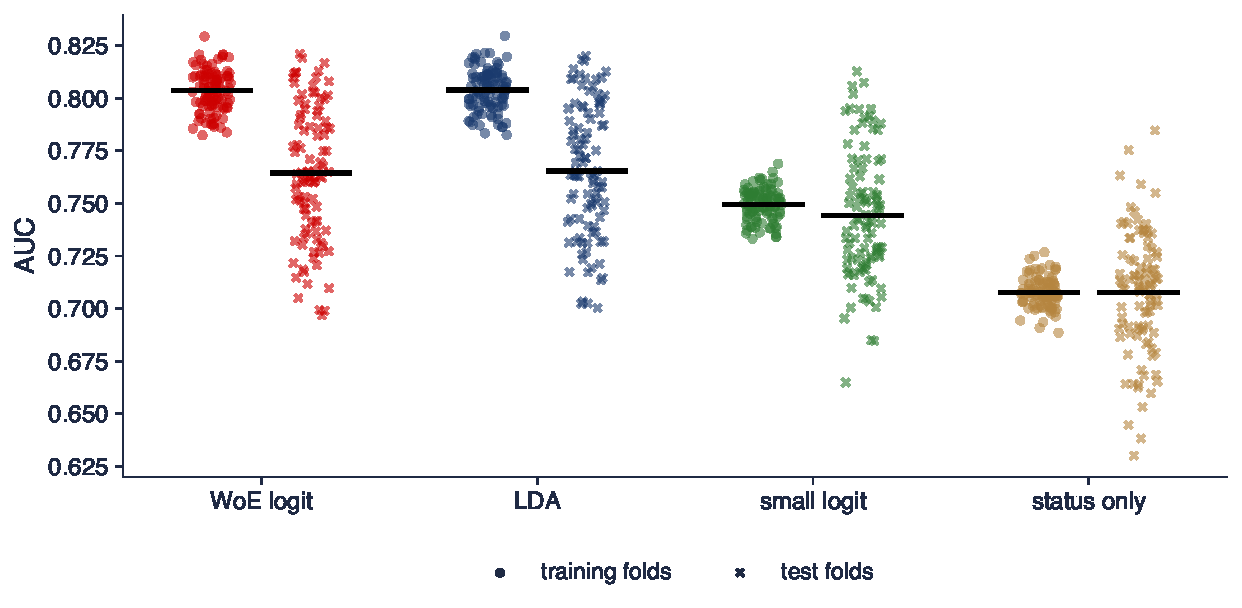
\includegraphics[width=0.97\textwidth,height=0.46\textheight,keepaspectratio]{sfm_ch12_cv_auc.pdf}
\end{center}
\vspace{-0.25cm}
\begin{itemize}
    \item 20 repetitions of 5 folds; dots: training folds, crosses: test folds; black lines: means
    \item WoE logit: training $0.804$, test $0.764$ (sd $0.032$); LDA: $0.804$, $0.765$; small logit: $0.749$, $0.744$; checking account: $0.708$
    \item Interpretation: the scorecard loses 0.039 AUC out of sample, the five-variable logit almost nothing; the single split above was lucky ($0.801$ against $0.764$ on average)
\end{itemize}
\sfmquantlet{Ch_12}{SFM_ch12_validation_irb}
\end{frame}

\begin{frame}{Out-of-Time Validation and Drift}
\itemsize{\small}
\begin{itemize}
    \item A scorecard is used for years on applicants who arrive \textbf{after} the estimation period
    \begin{itemize}
        \item the economy, the products and the applicants change: the relation between $x$ and default drifts
        \item out-of-time test: estimate on, say, 2019--2021, test on 2022--2023; compare AUC and calibration across years
    \end{itemize}
    \item Monitoring: the distribution of the scores and of each variable is compared with the training period
    \begin{itemize}
        \item a shift with stable ranking calls for recalibration (the constant); a loss of ranking calls for a new model
    \end{itemize}
    \item Data limitation: neither data set of this chapter has application dates, so an out-of-time test is not possible here; random splits are the most we can do
    \item Further reading, an out-of-time design for crypto ``zombie'' assets: \refPeleZ
\end{itemize}
\end{frame}

\begin{frame}{Case Study: Benchmarking Credit Scoring Methods}
\itemsize{\small}
\begin{itemize}
    \item \refLessmann: 41 classifiers, six accuracy measures, eight retail credit data sets (among them the German credit data of UCI)
    \begin{itemize}
        \item an update of the benchmark of Baesens et al.\ (2003), ten years later
    \end{itemize}
    \item Findings
    \begin{itemize}
        \item several classifiers predict significantly better than logistic regression, the industry standard; heterogeneous ensembles perform best
        \item more accurate scorecards can bring sizeable financial returns
        \item the common accuracy measures give similar signals; random forests are recommended as the benchmark for any new method
    \end{itemize}
    \item Beating the logit alone is no longer evidence of progress; on our 1000 credits, logit and LDA differ by less than one standard error of AUC; \sfmchlink{https://danpele.github.io/SFM/EN/Courses/chapter13_machine_learning.pdf}{Chapter 13} adds trees and neural networks
\end{itemize}
\end{frame}

\begin{frame}{Recap: Validation}
\itemsize{\small}
\begin{itemize}
    \item Discrimination: ROC, AUC, Gini $=$ AR, KS; calibration: reliability diagram, Hosmer--Lemeshow, Brier score
    \item Choose the cut-off from the costs, not from the accuracy
    \item Test out of sample, repeat with cross-validation, and test out of time whenever the data have dates
\end{itemize}
\end{frame}


%=============================================================================
\section{Reject Inference and Fairness}
%=============================================================================

\begin{frame}{Reject Inference}
\itemsize{\small}
\begin{itemize}
    \item The outcome is known only for \textbf{accepted} applicants; the model is used on \textbf{all} applicants (``through the door'')
    \begin{itemize}
        \item a sample selected by the old score: the riskiest applicants are missing, and so are their outcomes
        \item the South German Credit borrowers had all passed the bank's checks \refGroemping
    \end{itemize}
    \item \textbf{Reject inference}: methods that try to correct for the missing outcomes \refBCT; \refTCE
    \begin{itemize}
        \item reweighting: give accepted applicants who resemble the rejected ones a larger weight
        \item augmentation and parcelling: impute outcomes for the rejected from a model
        \item the most reliable source: a small random sample of applicants accepted regardless of the score
    \end{itemize}
\end{itemize}
\end{frame}

\begin{frame}{A Reject-Inference Experiment on the Taiwan Data}
\itemsize{\footnotesize}
\begin{itemize}
    \item An ``old score'' (late payment in September and the limit) accepts the best 70\% of the training clients (15\,085); their default rate is 13.2\%, that of the rejected 44.9\%
    \begin{itemize}
        \item among the accepted nobody was late in September: the strongest variable cannot be estimated and drops out
    \end{itemize}
    \item Test sample (all applicants): AUC of the model estimated on the accepted only $0.736$, on all applicants $0.777$, old score $0.743$
    \begin{itemize}
        \item rejected test clients: observed default rate 46.1\%; mean PD of the accepted-only model 29.6\%, of the full model 44.1\%
    \end{itemize}
    \item Interpretation: trained on the accepted only, the new model ranks worse than the old score and underestimates the risk of the rejected by about 36\%
\end{itemize}\sfmquantlet{Ch_12}{SFM_ch12_reject_fairness}
\end{frame}

\begin{frame}{Fairness in Credit Scoring}
\itemsize{\footnotesize}
\begin{columns}[T]
\begin{column}{0.62\textwidth}
\begin{itemize}
    \item US law forbids discrimination in credit by sex, marital status, race, religion, national origin or age \refECOA
    \begin{itemize}
        \item EU: credit scoring of persons is a high-risk use of AI (documentation, human oversight) \refAIAct
    \end{itemize}
    \item Leaving the protected variable out is not enough: other variables can stand in for it
    \begin{itemize}
        \item \textbf{demographic parity}: equal approval rates across groups
        \item \textbf{equal opportunity}: equal approval rates of the good payers \refHPS
        \item \textbf{calibration within groups}: the same PD means the same risk in every group
    \end{itemize}
    \item When default rates differ across groups, these criteria cannot all hold at once: the choice is a matter of policy for banks and regulators
\end{itemize}
\end{column}
\begin{column}{0.35\textwidth}
\centering
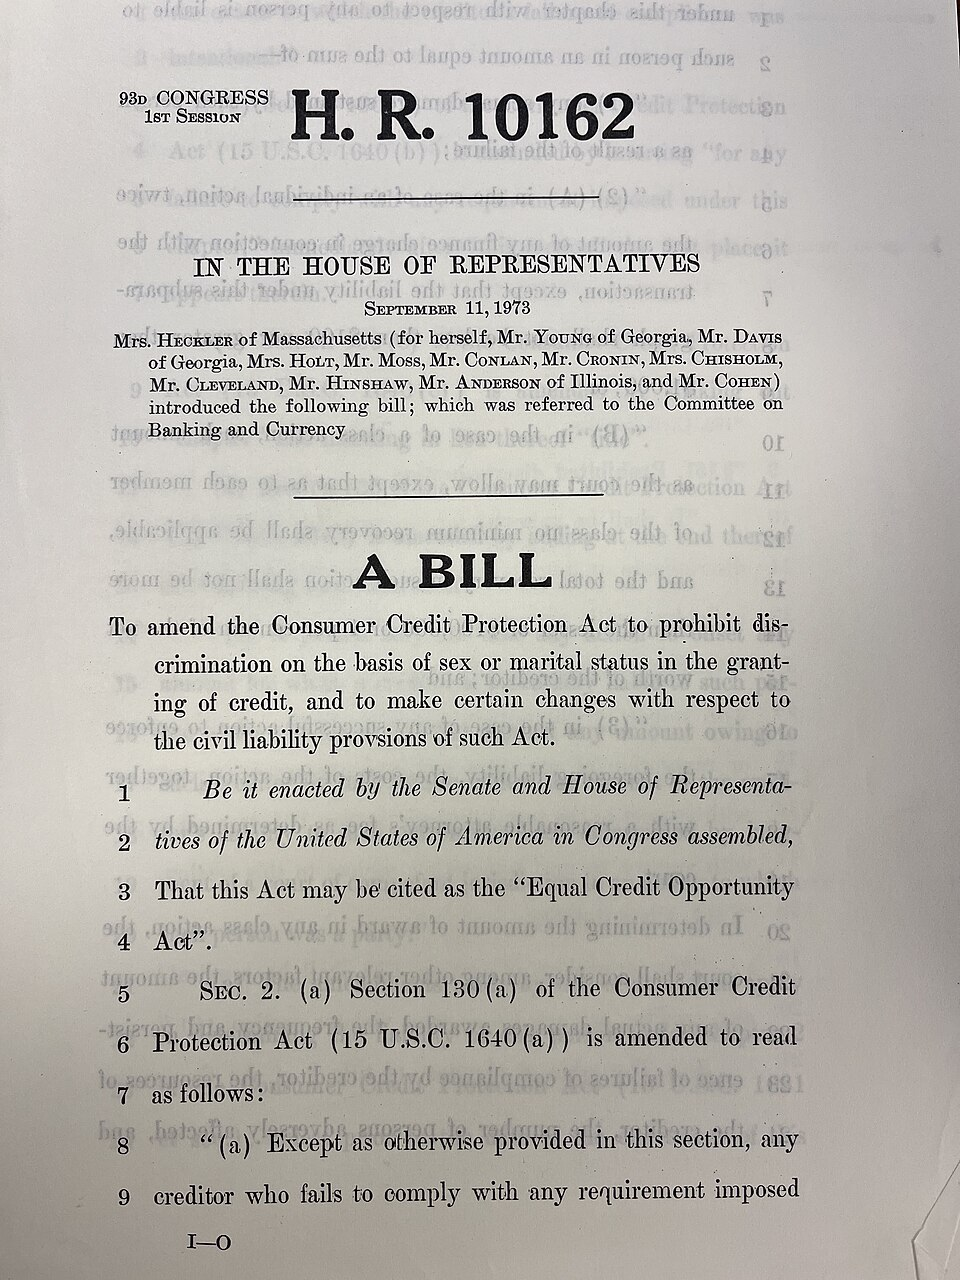
\includegraphics[height=0.46\textheight]{ch12_heckler_bill_1973.jpg}\\[1mm]
\imgcap{H.R. 10162 (1973), the bill that introduced the Equal Credit Opportunity Act}
\imgcredit{https://commons.wikimedia.org/wiki/File:A_Bill_to_amend_the_Consumer_Credit_Protection_Act.jpg}{Photo: H.R. 10162 (1973); public domain; Wikimedia Commons}
\end{column}
\end{columns}
\end{frame}

\begin{frame}{Approval and Default by Group: Taiwan}
\itemsize{\footnotesize}
\begin{center}
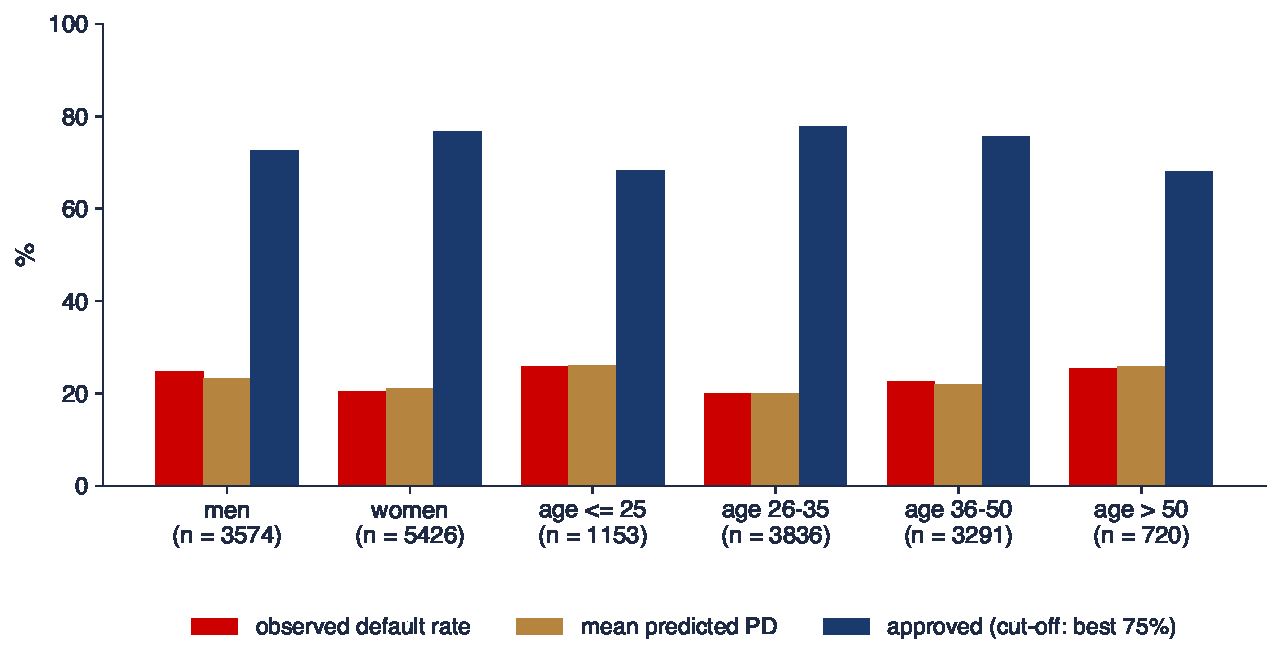
\includegraphics[width=0.97\textwidth,height=0.46\textheight,keepaspectratio]{sfm_ch12_fairness.pdf}
\end{center}
\vspace{-0.25cm}
\begin{itemize}
    \item Test sample; sex and age are not inputs of the model; cut-off: approve the 75\% with the lowest PD
    \item Women: default rate 20.5\%, approved 76.6\%; men: 24.7\%, 72.5\%; good payers approved: women 85.1\%, men 83.2\%
    \item Interpretation: the model is calibrated in every group (mean PD close to the observed rate), so groups with more defaults (men, the youngest and the oldest) are approved less often
\end{itemize}
\sfmquantlet{Ch_12}{SFM_ch12_reject_fairness}
\end{frame}

\begin{frame}{Case Study: Machine Learning and Unequal Credit}
\itemsize{\small}
\begin{itemize}
    \item \refFuster: US mortgages; default predicted with a traditional logit and with machine-learning models
    \begin{itemize}
        \item question: who gains and who loses when the lender switches to the more accurate model?
    \end{itemize}
    \item Findings
    \begin{itemize}
        \item the flexible models predict default better
        \item Black and Hispanic borrowers are less likely to gain from the new technology
        \item in an equilibrium model, the disparity in interest rates between and within groups increases, mainly because of the greater flexibility
    \end{itemize}
    \item Lesson: accuracy and fairness must be measured together; a better AUC is not a sufficient argument
\end{itemize}
\end{frame}

\begin{frame}{Recap: Reject Inference and Fairness}
\itemsize{\small}
\begin{itemize}
    \item Outcomes exist only for accepted applicants: a model trained on them extrapolates to the rejected
    \item Fairness criteria (parity, equal opportunity, calibration) conflict when base rates differ
    \item Removing a protected variable does not remove its influence
\end{itemize}
\end{frame}


%=============================================================================
\section{Corporate Default: Altman and Merton}
%=============================================================================

\begin{frame}{The Altman Z-Score (1968)}
\itemsize{\footnotesize}
\begin{columns}[T]
\begin{column}{0.60\textwidth}
\begin{itemize}
    \item \refAltman: 66 US manufacturing firms, 33 that filed for bankruptcy in 1946--1965 and 33 matched survivors
    \begin{itemize}
        \item Fisher's discriminant analysis on five accounting ratios
    \end{itemize}
    \item $Z = 1.2X_1 + 1.4X_2 + 3.3X_3 + 0.6X_4 + 1.0X_5$
    \begin{itemize}
        \item $X_1$ working capital / total assets (TA); $X_2$ retained earnings / TA; $X_3$ EBIT (earnings before interest and taxes) / TA
        \item $X_4$ market value of equity / book value of debt; $X_5$ sales / TA
        \item zones: $Z < 1.81$ distress, $1.81$--$2.99$ grey, $Z > 2.99$ safe
    \end{itemize}
    \item About 95\% of the sample correctly classified one year before bankruptcy; the accuracy falls quickly for longer horizons
\end{itemize}
\end{column}
\begin{column}{0.37\textwidth}
\centering

\includegraphics[height=0.36\textheight]{ch12_nyu_stern_2019.jpg}\\[1mm]
\imgcap{NYU Stern School of Business, Altman's institution}
\imgcredit{https://commons.wikimedia.org/wiki/File:NYU_Stern_School_of_Business_-_Henry_Kaufman_Management_Center_(48072761732).jpg}{Photo: Ajay Suresh (2019); CC BY 2.0; Wikimedia Commons}
\end{column}
\end{columns}
\end{frame}

\begin{frame}{Worked Example: a Z-Score}
\itemsize{\small}
\begin{itemize}
    \item A hypothetical firm: $X_1 = 0.15$, $X_2 = 0.20$, $X_3 = 0.08$, $X_4 = 0.90$, $X_5 = 1.10$
    \begin{itemize}
        \item $Z = 1.2 \times 0.15 + 1.4 \times 0.20 + 3.3 \times 0.08 + 0.6 \times 0.90 + 1.0 \times 1.10$
        \item $Z = 0.180 + 0.280 + 0.264 + 0.540 + 1.100 = 2.364$: the grey zone
    \end{itemize}
    \item Which ratio would move the firm to the safe zone?
    \begin{itemize}
        \item an EBIT/TA of 0.27 instead of 0.08 adds $3.3 \times 0.19 \approx 0.63$: $Z \approx 2.99$
    \end{itemize}
    \item Limits
    \begin{itemize}
        \item the weights come from 66 US manufacturers of 1946--1965; other sectors and countries need re-estimation
        \item Z is a discriminant score, not a PD; later models give PDs: logit \refOhlson, hazard models \refShumway
    \end{itemize}
\end{itemize}
\end{frame}

\begin{frame}{Merton's Distance to Default}
\itemsize{\footnotesize}
\begin{columns}[T]
\begin{column}{0.66\textwidth}
\begin{itemize}
    \item \refMerton: the value $V_t$ of the firm's assets follows a GBM (geometric Brownian motion, \sfmchlink{https://danpele.github.io/SFM/EN/Courses/chapter4_probability.pdf}{Chapter 4}) with drift $\mu$ and volatility $\sigma_V$
    \begin{itemize}
        \item debt with face value $D$ due at $T$; default if $V_T < D$; equity is a call option on the assets
    \end{itemize}
    \item $\ln V_T \sim N\big(\ln V_0 + (\mu - \sigma_V^2/2)T,\ \sigma_V^2T\big)$, so
    \begin{itemize}
        \item $\mathrm{DD} = \dfrac{\ln(V_0/D) + (\mu - \sigma_V^2/2)T}{\sigma_V\sqrt{T}}$, \quad $\mathrm{PD} = \Phi(-\mathrm{DD})$
        \item DD: the number of standard deviations between the expected asset value and the debt
    \end{itemize}
    \item $V$ and $\sigma_V$ are not observed: they are solved from the equity price and the equity volatility (option pricing)
\end{itemize}
\end{column}
\begin{column}{0.31\textwidth}
\centering

\includegraphics[height=0.42\textheight]{ch12_merton_2010.jpg}\\[1mm]
\imgcap{Robert C. Merton, 2010}
\imgcredit{https://commons.wikimedia.org/wiki/File:Robert_Merton_November_2010_(2x3_cropped).jpg}{Photo: Massachusetts Institute of Technology (2010); CC BY-SA 4.0; Wikimedia Commons}
\end{column}
\end{columns}
\end{frame}

\begin{frame}{Worked Example: Distance to Default}
\itemsize{\footnotesize}
\begin{itemize}
    \item $V_0 = 100$, $D = 70$, $\sigma_V = 25\%$, $\mu = 5\%$, $T = 1$ year
    \begin{itemize}
        \item $\ln(100/70) = 0.3567$; $\mu - \sigma_V^2/2 = 0.05 - 0.03125 = 0.01875$
        \item $\mathrm{DD} = 0.3754/0.25 = 1.502$; PD $= \Phi(-1.502) = 6.66\%$
    \end{itemize}
    \item From the market: equity 40, equity volatility 50\%, debt 70, risk-free rate 3\%
    \begin{itemize}
        \item solving $E = V\Phi(d_1) - De^{-rT}\Phi(d_2)$ and $\sigma_E E = \Phi(d_1)\sigma_V V$: $V = 107.9$, $\sigma_V = 18.6\%$, DD $= 2.39$, PD $= 0.84\%$
        \item $d_1$, $d_2$: the Black--Scholes terms of \sfmchlink{https://danpele.github.io/SFM/EN/Courses/chapter4_probability.pdf}{Chapter 4}, with $V$ in place of the share price
    \end{itemize}
    \item Interpretation: a market-based PD reacts every day to prices; an accounting score changes once a year
\end{itemize}\sfmquantlet{Ch_12}{SFM_ch12_altman_merton}
\end{frame}

\begin{frame}{Merton: Asset Paths and PD}
\itemsize{\footnotesize}
\begin{center}
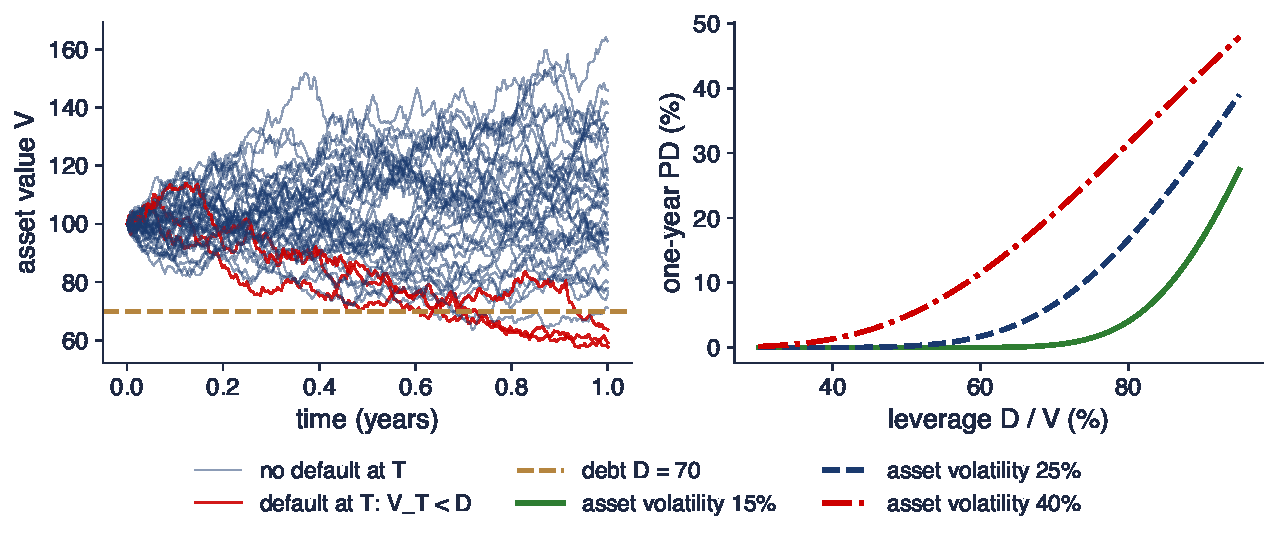
\includegraphics[width=0.97\textwidth,height=0.46\textheight,keepaspectratio]{sfm_ch12_merton.pdf}
\end{center}
\vspace{-0.25cm}
\begin{itemize}
    \item Left: 40 simulated asset paths ($V_0 = 100$, $\mu = 5\%$, $\sigma_V = 25\%$); red: the paths that end below the debt of 70
    \item Right: one-year PD against leverage $D/V$ for three asset volatilities
    \item Interpretation: PD is almost zero at low leverage and rises steeply between 70\% and 90\%; the higher the volatility, the earlier the rise
\end{itemize}
\sfmquantlet{Ch_12}{SFM_ch12_altman_merton}
\end{frame}

\begin{frame}{Case Study: How Good Is the Merton Model?}
\itemsize{\small}
\begin{itemize}
    \item \refBS: US firms; the Merton DD against a ``naive'' DD with the same functional form but without solving the model
    \begin{itemize}
        \item design: hazard models of default and out-of-sample forecasts; comparison with CDS (credit default swap) spreads and bond yields
    \end{itemize}
    \item Findings
    \begin{itemize}
        \item the naive DD performs slightly better than the Merton DD out of sample
        \item other variables (e.g.\ past returns) add information: DD is not a sufficient statistic for PD
        \item its functional form (leverage scaled by volatility) is what makes it useful
    \end{itemize}
    \item Lesson: theory gives a good variable, statistics decides how to use it; the same holds for the Z-score
\end{itemize}
\end{frame}

\begin{frame}{Recap: Altman and Merton}
\itemsize{\small}
\begin{itemize}
    \item Altman: LDA on five accounting ratios; zones 1.81 and 2.99
    \item Merton: equity is a call on the assets; DD $= [\ln(V/D) + (\mu - \sigma^2/2)T]/(\sigma\sqrt{T})$, PD $= \Phi(-\mathrm{DD})$
    \item Both are best used as inputs of a statistical PD model
\end{itemize}
\end{frame}


%=============================================================================
\section{AI for Scientific Discovery}
%=============================================================================

\begin{frame}{An Open Question}
\itemsize{\small}
\begin{itemize}
    \item \textbf{Do flexible machine-learning scores improve default prediction enough to justify their cost in transparency and fairness?}
    \begin{itemize}
        \item today: WoE logit and LDA reach a test AUC of about 0.764; benchmarks find significant gains for ensembles \refLessmann
        \item the gains may be unequal across groups \refFuster; support vector machines for default: \refCHM
    \end{itemize}
    \item Why it is open: gains depend on the data set, the measure and the population; the outcomes of rejected applicants are never seen
    \item AI tools can speed up such a study; they do not replace checking it \refWang
\end{itemize}
\end{frame}

\begin{frame}{How AI Could Help}
\itemsize{\small}
\begin{itemize}
    \item \textbf{Literature}: a list of benchmark studies of credit scoring and of studies on fairness in lending, with their data sets
    \item \textbf{Code}: a first draft of a cross-validated comparison of the WoE logit with gradient boosting on the Taiwan data
    \item \textbf{Robustness}: other cut-offs, other measures (Brier, cost), group-wise AUC and calibration
    \item Example prompt
    \begin{itemize}
        \item \aiprompt{Write Python code that compares a WoE logistic regression with gradient boosting on the Taiwan credit card default data by repeated stratified 5-fold cross-validation, recomputing the WoE bins inside each fold, and reports AUC, Brier score and the approval rates of men and women at a 75 percent approval cut-off.}
    \end{itemize}
\end{itemize}
\end{frame}

\begin{frame}{What to Check}
\itemsize{\small}
\begin{itemize}
    \item The coding of the outcome: default $= 1$; a reversed coding flips every sign and every curve
    \item The WoE sign convention: ln(goods/bads) here; some sources use ln(bads/goods)
    \item No leakage: bins, WoE and variable selection inside each training fold
    \item AUC is not accuracy, and Gini $= 2\,$AUC $- 1$, not AUC $- 0.5$
    \item PDs from an oversampled data set need the prior correction before any EL or capital number
    \item References: every cited paper and data set must exist; check the DOI
\end{itemize}
\end{frame}

\begin{frame}{Project Idea}
\itemsize{\small}
\begin{itemize}
    \item \textbf{Question}: on the Taiwan credit card data, how much AUC does gradient boosting add over the WoE logit, and what happens to the approval rates by sex and age?
    \begin{itemize}
        \item data: \refTW{} (CC BY 4.0), saved in data/credit
    \end{itemize}
    \item Steps
    \begin{itemize}
        \item WoE bins and IV for every variable; a WoE logit; gradient boosting with default settings
        \item repeated stratified cross-validation: AUC with DeLong intervals, Brier score, calibration
        \item fairness at one cut-off: demographic parity and equal opportunity for sex and age groups
    \end{itemize}
    \item Deliverable: one table, one chart, and a paragraph on what the data can and cannot show
    \item Declare any AI use, and list the errors of the AI that you corrected
\end{itemize}
\end{frame}


%=============================================================================
\section{Summary}
%=============================================================================

\begin{frame}{Key Takeaways}
\itemsize{\small}
\begin{itemize}
    \item EL $=$ PD $\times$ LGD $\times$ EAD is priced in; IRB capital covers the unexpected loss
    \item WoE turns every variable into log-odds evidence; IV ranks the variables
    \item Logit: $e^{\beta}$ is an odds ratio; LDA (Fisher) gives the same linear log-odds under Normality and ranks equally well here
    \item A scorecard: Score $=$ Offset $+$ Factor $\ln$(good:bad odds), PDO $= 20$ points per doubling
    \item Validate discrimination (AUC, Gini, KS) and calibration (Brier, reliability diagram) out of sample; choose the cut-off from costs
    \item Rejected applicants and protected groups need explicit checks; Altman and Merton add accounting and market information
\end{itemize}
\end{frame}

\begin{frame}{Key Formulas}
\itemsize{\small}
{\renewcommand{\arraystretch}{1.4}\begin{center}
\scriptsize
\begin{tabular}{ll}
\toprule
\textbf{Quantity} & \textbf{Formula} \\
\midrule
EL & $\mathrm{PD} \times \mathrm{LGD} \times \mathrm{EAD}$ \\
WoE, IV & $\ln\frac{g_i/G}{b_i/B}$, \ $\sum_i (g_i/G - b_i/B)\,\mathrm{WoE}_i$ \\
Logit & $\ln\frac{p}{1 - p} = \beta_0 + x^\top\beta$, \ $p = 1/(1 + e^{-\eta})$ \\
LDA & $w = S_W^{-1}(m_1 - m_0)$ \\
Prior correction & $+\ln\frac{\pi/(1 - \pi)}{\pi_s/(1 - \pi_s)}$ to the constant \\
Scorecard & $\text{Offset} + \frac{\text{PDO}}{\ln 2}\ln\frac{1 - p}{p}$ \\
AUC, Gini & $P(s_{\text{bad}} > s_{\text{good}})$, \ $2\,\mathrm{AUC} - 1$ \\
KS, Brier & $\max_s|F_1(s) - F_0(s)|$, \ $\frac1n\sum(p_i - y_i)^2$ \\
Bayes cut-off & $p > C_{FP}/(C_{FP} + C_{FN})$ \\
Merton & $\mathrm{DD} = \frac{\ln(V/D) + (\mu - \sigma^2/2)T}{\sigma\sqrt{T}}$, \ $\mathrm{PD} = \Phi(-\mathrm{DD})$ \\
\bottomrule
\end{tabular}
\end{center}
}
\end{frame}

\begin{frame}{Check Yourself}
\itemsize{\small}
\begin{itemize}
    \item \textbf{Question}: a model has an accuracy of 70\% on the South German Credit test sample. Is it good?
    \begin{itemize}
        \item \textbf{Answer}: not necessarily: ``everybody is good'' already reaches 70\%; look at AUC, TPR, FPR and the cost
    \end{itemize}
    \item \textbf{Question}: the coefficient of a dummy in a logit is 0.69. What does it mean?
    \begin{itemize}
        \item \textbf{Answer}: the odds of default are multiplied by $e^{0.69} \approx 2$ for the group, relative to the reference group
    \end{itemize}
    \item \textbf{Question}: does correcting the PDs for oversampling change the AUC?
    \begin{itemize}
        \item \textbf{Answer}: no: it shifts all log-odds by the same constant, so the ranking is unchanged
    \end{itemize}
    \item Next: \sfmchlink{https://danpele.github.io/SFM/EN/Courses/chapter13_machine_learning.pdf}{Chapter 13}, machine learning
\end{itemize}
\end{frame}


%=============================================================================
\section{References}
%=============================================================================

\begin{frame}{References (1/2)}
\itemsize{\tiny}
\begin{itemize}
    \item Altman, E.I. (1968). \href{https://doi.org/10.1111/j.1540-6261.1968.tb00843.x}{Financial ratios, discriminant analysis and the prediction of corporate bankruptcy}. \textit{Journal of Finance}, 23(4), 589--609.
    \item Banasik, J., Crook, J., Thomas, L. (2003). \href{https://doi.org/10.1057/palgrave.jors.2601578}{Sample selection bias in credit scoring models}. \textit{Journal of the Operational Research Society}, 54(8), 822--832.
    \item Basel Committee on Banking Supervision (2005). \href{https://www.bis.org/bcbs/irbriskweight.htm}{An explanatory note on the Basel II IRB risk weight functions}. Bank for International Settlements.
    \item Basel Committee on Banking Supervision (2006). \href{https://www.bis.org/publ/bcbs128.htm}{International convergence of capital measurement and capital standards: a revised framework (comprehensive version)}. Bank for International Settlements.
    \item Będowska-Sójka, B., Wójcik, P., Pele, D.T. (2026). \href{https://doi.org/10.1016/j.najef.2025.102543}{Early warning systems for cryptocurrency markets: predicting `zombie' assets using machine learning}. \textit{North American Journal of Economics and Finance}, 102543.
    \item Bharath, S.T., Shumway, T. (2008). \href{https://doi.org/10.1093/rfs/hhn044}{Forecasting default with the Merton distance to default model}. \textit{Review of Financial Studies}, 21(3), 1339--1369.
    \item Brier, G.W. (1950). \href{https://doi.org/10.1175/1520-0493(1950)078<0001:VOFEIT>2.0.CO;2}{Verification of forecasts expressed in terms of probability}. \textit{Monthly Weather Review}, 78(1), 1--3.
    \item Chen, S., Härdle, W.K., Moro, R.A. (2011). \href{https://doi.org/10.1080/14697680903410015}{Modeling default risk with support vector machines}. \textit{Quantitative Finance}, 11(1), 135--154.
    \item Cox, D.R. (1958). \href{https://doi.org/10.1111/j.2517-6161.1958.tb00292.x}{The regression analysis of binary sequences}. \textit{Journal of the Royal Statistical Society, Series B}, 20(2), 215--232.
    \item Default of Credit Card Clients [data set] (2009). \href{https://doi.org/10.24432/C55S3H}{UCI Machine Learning Repository}, CC BY 4.0.
    \item DeLong, E.R., DeLong, D.M., Clarke-Pearson, D.L. (1988). \href{https://doi.org/10.2307/2531595}{Comparing the areas under two or more correlated receiver operating characteristic curves: a nonparametric approach}. \textit{Biometrics}, 44(3), 837--845.
    \item Durand, D. (1941). \href{https://www.nber.org/books-and-chapters/risk-elements-consumer-instalment-financing-technical-edition}{\textit{Risk Elements in Consumer Instalment Financing}}, technical edition. National Bureau of Economic Research.
    \item European Commission (2024). \href{https://digital-strategy.ec.europa.eu/en/policies/regulatory-framework-ai}{AI Act: regulatory framework on artificial intelligence}. Shaping Europe's digital future.
    \item Federal Trade Commission. \href{https://www.ftc.gov/legal-library/browse/statutes/equal-credit-opportunity-act}{Equal Credit Opportunity Act}, 15 U.S.C. §§ 1691--1691f.
    \item Fisher, R.A. (1936). \href{https://doi.org/10.1111/j.1469-1809.1936.tb02137.x}{The use of multiple measurements in taxonomic problems}. \textit{Annals of Eugenics}, 7(2), 179--188.
    \item Franke, J., Härdle, W.K., Hafner, C.M. (2019). \href{https://doi.org/10.1007/978-3-030-13751-9}{\textit{Statistics of Financial Markets: An Introduction}}, 5th ed. Springer.
    \item Fuster, A., Goldsmith-Pinkham, P., Ramadorai, T., Walther, A. (2022). \href{https://doi.org/10.1111/jofi.13090}{Predictably unequal? The effects of machine learning on credit markets}. \textit{Journal of Finance}, 77(1), 5--47.
\end{itemize}
\end{frame}

\begin{frame}{References (2/2)}
\itemsize{\tiny}
\begin{itemize}
    \item Gordy, M.B. (2003). \href{https://doi.org/10.1016/S1042-9573(03)00040-8}{A risk-factor model foundation for ratings-based bank capital rules}. \textit{Journal of Financial Intermediation}, 12(3), 199--232.
    \item Grömping, U. (2019). \href{http://www1.beuth-hochschule.de/FB_II/reports/Report-2019-004.pdf}{South German credit data: correcting a widely used data set}. Reports in Mathematics, Physics and Chemistry 4/2019, Beuth University of Applied Sciences Berlin.
    \item Hand, D.J., Henley, W.E. (1997). \href{https://doi.org/10.1111/j.1467-985X.1997.00078.x}{Statistical classification methods in consumer credit scoring: a review}. \textit{Journal of the Royal Statistical Society, Series A}, 160(3), 523--541.
    \item Hanley, J.A., McNeil, B.J. (1982). \href{https://doi.org/10.1148/radiology.143.1.7063747}{The meaning and use of the area under a receiver operating characteristic (ROC) curve}. \textit{Radiology}, 143(1), 29--36.
    \item Härdle, W.K., Simar, L. (2019). \href{https://doi.org/10.1007/978-3-030-26006-4}{\textit{Applied Multivariate Statistical Analysis}}, 5th ed. Springer.
    \item Hardt, M., Price, E., Srebro, N. (2016). \href{https://arxiv.org/abs/1610.02413}{Equality of opportunity in supervised learning}. \textit{Advances in Neural Information Processing Systems} 29; arXiv:1610.02413.
    \item Hosmer, D.W., Lemeshow, S. (1980). \href{https://doi.org/10.1080/03610928008827941}{Goodness of fit tests for the multiple logistic regression model}. \textit{Communications in Statistics -- Theory and Methods}, 9(10), 1043--1069.
    \item Lessmann, S., Baesens, B., Seow, H.-V., Thomas, L.C. (2015). \href{https://doi.org/10.1016/j.ejor.2015.05.030}{Benchmarking state-of-the-art classification algorithms for credit scoring: an update of research}. \textit{European Journal of Operational Research}, 247(1), 124--136.
    \item Merton, R.C. (1974). \href{https://doi.org/10.1111/j.1540-6261.1974.tb03058.x}{On the pricing of corporate debt: the risk structure of interest rates}. \textit{Journal of Finance}, 29(2), 449--470.
    \item myFICO. \href{https://www.myfico.com/credit-education/blog/history-of-the-fico-score}{The history of the FICO score}. Fair Isaac Corporation.
    \item Ohlson, J.A. (1980). \href{https://doi.org/10.2307/2490395}{Financial ratios and the probabilistic prediction of bankruptcy}. \textit{Journal of Accounting Research}, 18(1), 109--131.
    \item Shumway, T. (2001). \href{https://doi.org/10.1086/209665}{Forecasting bankruptcy more accurately: a simple hazard model}. \textit{Journal of Business}, 74(1), 101--124.
    \item Siddiqi, N. (2006). \href{https://doi.org/10.1002/9781119201731}{\textit{Credit Risk Scorecards: Developing and Implementing Intelligent Credit Scoring}}. Wiley.
    \item South German Credit [data set] (2020). \href{https://doi.org/10.24432/C5QG88}{UCI Machine Learning Repository}, CC BY 4.0.
    \item Thomas, L.C., Crook, J., Edelman, D. (2017). \href{https://doi.org/10.1137/1.9781611974560}{\textit{Credit Scoring and Its Applications}}, 2nd ed. SIAM.
    \item Wang, H., Fu, T., Du, Y., Gao, W., et al. (2023). \href{https://doi.org/10.1038/s41586-023-06221-2}{Scientific discovery in the age of artificial intelligence}. \textit{Nature}, 620, 47--60.
    \item Yeh, I.-C., Lien, C.-H. (2009). \href{https://doi.org/10.1016/j.eswa.2007.12.020}{The comparisons of data mining techniques for the predictive accuracy of probability of default of credit card clients}. \textit{Expert Systems with Applications}, 36(2), 2473--2480.
\end{itemize}
\end{frame}

\end{document}
